%%%%%%%%%%%%%%%%%%%%%%%%%%%%%%%%%%%%%%%%%
% Short Sectioned Assignment LaTeX Template Version 1.0 (5/5/12)
% This template has been downloaded from: http://www.LaTeXTemplates.com
% Original author:  Frits Wenneker (http://www.howtotex.com)
% License: CC BY-NC-SA 3.0 (http://creativecommons.org/licenses/by-nc-sa/3.0/)
%%%%%%%%%%%%%%%%%%%%%%%%%%%%%%%%%%%%%%%%%

% \documentclass[paper=a4, fontsize=11pt]{scrartcl} % A4 paper and 11pt font size
\documentclass[11pt, a4paper]{book}
\usepackage[T1]{fontenc} % Use 8-bit encoding that has 256 glyphs
\usepackage[utf8]{inputenc}
\usepackage{fourier} % Use the Adobe Utopia font for the document - comment this line to return to the LaTeX default
\usepackage{listings} % para insertar código con formato similar al editor
\usepackage[spanish, es-tabla]{babel} % Selecciona el español para palabras introducidas automáticamente, p.ej. "septiembre" en la fecha y especifica que se use la palabra Tabla en vez de Cuadro
\usepackage{url} % ,href} %para incluir URLs e hipervínculos dentro del texto (aunque hay que instalar href)
\usepackage{graphics,graphicx, float, adjustbox} %para incluir imágenes y colocarlas
\usepackage[gen]{eurosym} %para incluir el símbolo del euro
\usepackage{cite} %para incluir citas del archivo <nombre>.bib
\usepackage{enumerate}
\usepackage{hyperref}
\usepackage{graphicx}
\usepackage{tabularx}
\usepackage{booktabs}
\usepackage{longtable}

\usepackage[table,xcdraw]{xcolor}
\hypersetup{
	colorlinks=true,	% false: boxed links; true: colored links
	linkcolor=black,	% color of internal links
	urlcolor=cyan		% color of external links
}
\renewcommand{\familydefault}{\sfdefault}
\usepackage{fancyhdr} % Custom headers and footers
\pagestyle{fancyplain} % Makes all pages in the document conform to the custom headers and footers
\fancyhead[L]{} % Empty left header
\fancyhead[C]{} % Empty center header
\fancyhead[R]{Jesús Miguel Jaldo Ruiz} % My name
\fancyfoot[L]{} % Empty left footer
\fancyfoot[C]{} % Empty center footer
\fancyfoot[R]{\thepage} % Page numbering for right footer
%\renewcommand{\headrulewidth}{0pt} % Remove header underlines
\renewcommand{\footrulewidth}{0pt} % Remove footer underlines
\setlength{\headheight}{13.6pt} % Customize the height of the header

\usepackage{titlesec, blindtext, color}
\definecolor{gray75}{gray}{0.75}
\newcommand{\hsp}{\hspace{20pt}}
\titleformat{\chapter}[hang]{\Huge\bfseries}{\thechapter\hsp\textcolor{gray75}{|}\hsp}{0pt}{\Huge\bfseries}
\setcounter{secnumdepth}{4}
\usepackage[Lenny]{fncychap}
\usepackage[table]{xcolor} 
\setlength{\parskip}{2mm}

\begin{document}

	% Plantilla portada UGR
	\begin{titlepage}
\newlength{\centeroffset}
\setlength{\centeroffset}{-0.5\oddsidemargin}
\addtolength{\centeroffset}{0.5\evensidemargin}
\thispagestyle{empty}

\noindent\hspace*{\centeroffset}\begin{minipage}{\textwidth}

\centering

\includegraphics[width=0.9\textwidth]{logos/logo_ugr.jpg}\\[1.4cm]

\textsc{ \Large TRABAJO FIN DE GRADO\\[0.2cm]}
\textsc{ GRADO EN INGENIERIA INFORMATICA}\\[1cm]

{\Huge\bfseries Covid-19 Reports \\}
\noindent\rule[-1ex]{\textwidth}{3pt}\\[3.5ex]
{\large\bfseries Visualización personalizada de datos del COVID-19 }
\end{minipage}

\vspace{2.5cm}
\noindent\hspace*{\centeroffset}
\begin{minipage}{\textwidth}
\centering

\textbf{Autor}\\ {Jesús Miguel Jaldo Ruiz}\\[2.5ex]
\textbf{Director}\\ {Juan Julián Merelo Guervós}\\[2cm]

\includegraphics[width=0.3\textwidth]{logos/etsiit_logo.png}\\[0.1cm]
\textsc{Escuela Técnica Superior de Ingenierías Informática y de Telecomunicación}\\
\textsc{---}\\
Granada, Noviembre de 2020
\end{minipage}
\end{titlepage}


	% Plantilla prefacio UGR
	\thispagestyle{empty}

\begin{center}
{\large\bfseries Covid-19 Reports \\ Visualización personalizada de datos del COVID-19 }\\
\end{center}
\begin{center}
Jesús Miguel Jaldo Ruiz\\
\end{center}

%\vspace{0.7cm}

\vspace{0.5cm}
\noindent{\textbf{Palabras clave}: \textit{software libre, Covid-19, pandemia, virus, dispositivo movil, Telegram, Bot, Scrum}
\vspace{0.7cm}

\noindent{\textbf{Resumen}\\

El trabajo que se realiza en este proyecto consiste en el desarrollo de una aplicación que permita a los usuarios la consulta de datos sobre el Covid-19 en España y sus Comunidades Autónomas.

La aplicación se presentará con un entorno sencillo e interactivo donde los usuarios podrán, mediante el uso de botones, realizar diferentes consultas de datos, los cuales se mostrarán acompañados de una gráfica relacionada con los mismos. Ejemplos de estos datos son: la incidencia acumulada, el nº de fallecidos por el virus, los datos de hospitalización, etc.

\cleardoublepage

\begin{center}
	{\large\bfseries Covid-19 Reports \\ Customized display of COVID-19 data}\\
\end{center}
\begin{center}
Jesús Miguel Jaldo Ruiz\\
\end{center}
\vspace{0.5cm}
\noindent{\textbf{Keywords}: \textit{open source, Covid-19, pandemic, virus, movile device, Telegram, Bot, Scrum}, \textit{floss}
\vspace{0.7cm}

\noindent{\textbf{Abstract}\\

This proyect consist in the development of an application that allows users to consult data about the Covid-19 in Spain and its Autonomous Communities.

The application will have a simple and interactive environment where users will press buttons to perform different data queries, which will be shown with a graph related to them. Examples of these data are: the accumulated incidence, the number of deaths from the virus, hospitalization data, etc.

\cleardoublepage

\thispagestyle{empty}

\noindent\rule[-1ex]{\textwidth}{2pt}\\[4.5ex]

D. \textbf{Juan Julián Merelo Guervós}, Profesor(a) del ...

\vspace{0.5cm}

\textbf{Informo:}

\vspace{0.5cm}

Que el presente trabajo, titulado \textit{\textbf{Covid-19 Reports. Visualización personalizada de datos del COVID-19}},
ha sido realizado bajo mi supervisión por \textbf{Jesús Miguel Jaldo Ruiz}, y autorizo la defensa de dicho trabajo ante el tribunal
que corresponda.

\vspace{0.5cm}

Y para que conste, expiden y firman el presente informe en Granada a Noviembre de 2020.

\vspace{1cm}

\textbf{El director: }

\vspace{5cm}

\noindent \textbf{Juan Julián Merelo Guervós}

\chapter*{Agradecimientos}

A mi familia

A mis amigos

A mi escuela y sus profesores


	% Índice de contenidos
	\newpage
	\tableofcontents

	% Índice de imágenes y tablas
	\newpage
	\listoffigures

	% Si hay suficientes se incluirá dicho índice
	\listoftables 
	\newpage

	% Introducción 
	\chapter{Introducción} \label{ch:introduccion}

Este proyecto es software libre, y está liberado con la licencia \cite{agplv3}.

\section{Motivación}

Vivimos en tiempos extraños, desde diciembre de 2019 escuchamos hablar sobre la aparición de un brote epidemiológico de neumonía cuya causa era desconocida por aquel entonces en la ciudad china de Wuhan. Este brote tuvo lugar en el mercado de la ciudad y tras el aviso de las autoridades competentes de Wuhan a la OMS (Organización Mundial de la Salud) se empezó a investigar que podría estar provocando dicho brote. Esto hizo que tras varias investigaciones se conociera que la causa del mismo era la aparición de un nuevo coronavirus \cite{oms-covid} de tipo zoonótico; al cual se le dio el nombre de Covid-19. Según declaraciones de la OMS, este virus presentaba un riesgo para la salud pública, bajo las regulaciones del Reglamento Sanitario Internacional \cite{reglamento-sanitario-internacional} y posteriormente este sería considerado como una pandemia.

Poco a poco este nuevo virus fue extendiéndose, empezando por el continente asiático y por el resto del planeta.Todos y cada uno de los países afectados han aportado los datos de las diferentes incidencias que ha tenido el virus dentro de sus fronteras, aunque a pesar de ello seguimos sin conocer el alcance real de la pandemia ya que no existe un criterio común para la publicación de los datos, si no que cada país los calcula siguiendo los métodos que considera oportunos, por lo que la incidencia puede ser incluso mayor de lo mostrado por los datos, pero no vamos a centrarnos en como se calculan dichos datos.

Basándonos en esto, sabemos que existe una preocupación por parte de la población hacia el virus, a la cual le gusta estar informada. Hoy en día es importante estar bien informado, como nos muestra Gabriela Nova en su articulo "Los beneficios de estar informado" \cite{gabriela-nova}. Por ello, la mayor preocupación de la gente es conocer información a cerca del virus, de como está evolucionando, cuantas contagios, muertes y altas se han producido, entre otros datos. Podemos comprobar que actualmente el Covid-19 es una de las principales preocupaciones de la población, algunas de ellas que aparecen como consecuencia del propio virus. La Figura \ref{fig:preocupaciones} refleja una tabla con las preocupaciones principales de la población, donde se puede apreciar que el Covid-19 es la segunda preocupación de los españoles.

\begin{figure}[htb]
	\centering
	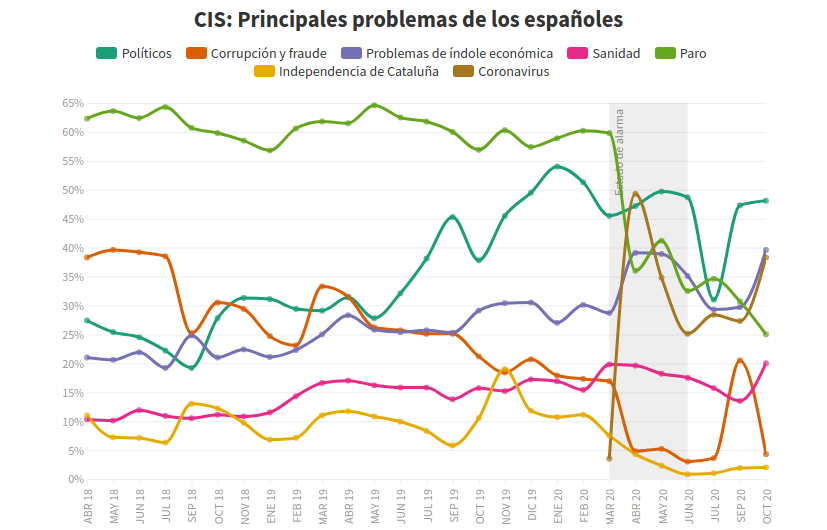
\includegraphics[width=1\textwidth]{img/preocupaciones}
	\caption{Preocupaciones de la población española. Fuente: \cite{rtve-preocupaciones}}
	\label{fig:preocupaciones}
\end{figure}

Como hemos dicho, a la gente le gusta estar informada, y más ahora, por lo que la transparencia en una situación como la que se está viviendo es algo más que esencial. Esta información tiene como funcionalidad mantener a la gente tranquila, pudiendo aportarles datos de la evolución de la pandemia, pero no solo eso, si no que también sirven para hacer un análisis de cara a la implementación y toma de medidas por parte de los gobiernos de los países afectados. Sin embargo todos estos datos a pesar de ser accesibles para la población, presentan un problema, la difícil visualización de esto de una manera sencilla e intuitiva. En este punto podemos hacernos una pregunta: ¿como podemos ofrecer esa información de manera que pueda ser útil a toda la población que quiera consultar y hacer uso de ella?

La respuesta a la pregunta anterior podemos decir que puede llegar a ser obvia en los tiempos en los que vivimos, donde la tecnología se ha instalado para quedarse en nuestra vida, por lo que podríamos decir que la respuesta a nuestra pregunta es: hacer uso de la tecnología. Los smartphones es un producto que hoy en día todo el mundo tiene, según la web Stadista \cite{statista}, en 2019 alrededor de los 2.650 millones de usuarios cuentan con uno. Para ser mas concretos el 96\% de los ciudadanos españoles mayores de 14 años que acceden a internet lo hacen desde su smartphone. De la misma forma un 92\% usa el móvil todos los días en una media de 3 horas diarias según el siguiente artículo \cite{elperiodico}.

\section{Alcance}

Este proyecto está pensado para poder llegar a una gran número de usuarios de todo el país. Lo que se pretende es que sean los propios usuarios los encargados de dar a conocer el proyecto. Sabemos que a veces el propio boca a boca es una de las maneras más eficaces de propagación, y en la época en la que nos situamos las personas suelen buscar recomendaciones sobre los productos que van a consumir o utilizar. Si tu como usuario estas contento con la aplicación se la recomendarás a más gente de tu entorno, lo que provocará no solo un aumento de usuarios, ya que estos se lo dirán a su vez a otros, con el fin de conseguir llegar al máximo número de personas posibles, proporcionándole información sobre la enfermedad.

Como hemos mencionado al inicio, toda la información puede ser consultada por la propia población, ¿entonces que sentido tiene este proyecto?. Entre otras cosas, cada Comunidad Autonómica tiene su propia manera de publicar los datos, a veces de una manera más sencilla y otras de una manera más compleja. Por ello lo que se pretende con \textbf{Covid-19 Reports} es poder agrupar toda esta información en un mismo lugar, facilitando el acceso a los usuarios y mostrando información adicional, por ejemplo, gráficos de la evolución de los datos seleccionados.

\section{Objetivos generales}

El objetivo principal de este proyecto es el desarrollo de un bot móvil orientado a informar a la población española para poder conocer los datos más relevantes sobre la pandemia del Covid-19 de una manera fiable. Este nos permitirá la consulta, tanto a nivel de todo el país como de las diferentes Comunidades Autónomas, de datos como el incremento de los casos desde el inicio de la pandemia, los casos registrados las últimas 24 horas, el número de fallecidos, los datos hospitalarios, etc.

Para llevar a cabo el proyecto se pondrá en práctica la metodología de desarrollo Scrum, la cual usaremos para la planificación y desarrollo del proyecto, con el fin de aprovechar las ventajas que esta nos ofrece.

Está claro, como hemos dicho antes, que una de las mayores preocupaciones de la población es el Covid-19, Por ello, \textbf{Covid-19 Reports} se ha llevado a cabo con el fin de evitar una desinformación en cuanto a los datos y la evolución de esta pandemia se refieren, estando de forma libre y accesible para todos lo usuarios que así quieran hacer uso de ella.

También es cierto, que estos mismos datos ya pueden ser consultados en diferentes lugares, como son las webs de los propios organismos de gobiernos, pero también lo es que cada organismo adapta esos datos y su acceso según ellos crean convenientes y adaptándose a estructuras en sus webs que ya disponían. Por todo ello, otro de los objetivos de este bot es la de no solo unificar, si no la de mostrar de una forma sencilla e idéntica los datos, evitando tener que aprender a como acceder a los datos o evitar la confusión del usuario si desea consultar los datos de otra comunidad, bien por ver la evolución, o bien para conocer la situación en todas las Comunidades Autónomas del país.

	% Estado del arte
	% 	1. Crítica al estado del arte
	% 	2. Propuesta
	\chapter{Estado del arte} \label{ch:estado_del_arte}

En este apartado lo que pretende es mostrar como se encuentra el panorama en el cual vamos a llevar a cabo nuestro proyecto. Para ello, en primer lugar realizaremos un análisis del mercado, donde se presentarán las principales alternativas a nuestra idea de proyecto ya existentes, de forma que analicemos los requisitos de nuestro sistema comparándolo con los de aquellos que ya existen. En segundo lugar analizaremos punto por punto los recursos utilizados para poder llevar a cabo este proyecto.

\section{Análisis de mercado}

En el Capítulo~\ref{ch:introduccion} comentábamos que el acceso a los datos ya era algo posible para toda la población. Esto se debe a que son de dominio público y es el propio gobierno de España o las Comunidades Autónomas los que publican los datos en sus respectivas web. Dado que este proyecto está centrado en la visualización de datos, es muy importante poder realizar una comparación de los requisitos que queremos presentar en el mismo con las diversas funcionalidades de otras aplicaciones englobadas dentro del mismo género. Por desgracia, tras realizar una búsqueda de aplicaciones en la \textbf{Play Store} de Google a fecha de Noviembre de 2020, el resultado mostrado a sido bastante sorprendente. Según \textbf{Play Store}, no hay ningún tipo de aplicación similar a lo que se pretende desarrollar en este proyecto. Ejemplo de ello son las aplicaciones que nos sugiere:

\begin{itemize}
	\item \textbf{Radar COVID:} Aplicación de alertas en caso de haber estado cerca de alguien que tiene COVID-19
	\item \textbf{GVA Coronavirus:} Aplicación de la Generalitat Valenciana para solicitar citas en caso de mostrar síntomas.
	\item \textbf{PassCOVIS.gal} Aplicación de la Xunta de Galicia para recibir avisos, información de las restricciones, recomendaciones y novedades.
	\item \textbf{COVIS-19.eus} Aplicación del Gobierno del País Vasco para realizar un auto-diagnóstico y avisar a tu círculo de personas.
	\item \textbf{CONFINAPP} Aplicación que pretende ser un acompañamiento y la puerta de entrada a la información y servicios de la Generalitat de Cataluña.
\end{itemize}

Visto que en el ámbito de las aplicaciones móviles no encontramos nada similar, tendremos que hacer una comparación con la principal fuente actual de información de la que disponemos, el \textbf{Gobierno de España}.

En este punto, antes que hacer el análisis, debemos conocer cuales son los requisitos que queremos tener en nuestra aplicación. Tras un estudio de los datos, siguiendo un criterio propio, he recogido las funcionalidades principales con las que debería contar una aplicación como la que se va a desarrollar y que permitan al propio usuario tener acceso a la misma sin ningún conocimiento previo. Estas funcionalidades por consiguiente sí están presentes en \textbf{Covid-19 Reports} y son las siguientes:

\begin{enumerate}
	\item Seleccionar la Comunidad Autónoma sobre la que se quieren conocer los datos.
	\item Visualización del incremento de casos, casos acumulados, media de la última semana y últimas 24h.
	\item Visualización de los fallecimientos acumulados, media de la última semana y últimas 24 horas.
	\item Visualización de los datos de hospitalización, camas y camas UCI ocupadas, porcentaje del total de camas, altas e ingresos.
	\item Visualización de casos y muertes según la edad, solo al consultar datos de España.
	\item Visualización de los casos por cada 100mil habitantes, solo al consultar datos de España.
	\item Visualización de los casos por cada 100mil habitantes en la última semana, solo al consultar datos de España.
	\item Visualización de los fallecidos por cada 100mil habitantes, solo al consultar datos de España.
	\item Visualización de los fallecidos por cada 100mil habitantes en la última semana, solo al consultar datos de España.
	\item Visualización ordenada y clara.
	\item Toda la información es gratuita.
	\item No tiene ampliaciones de pago.
	\item No tiene anuncios.
	\item Plataforma móvil donde se ofrece
\end{enumerate}

\subsection{Representación de datos Covid-19 en España}

Como hemos dicho antes, llevaremos a cabo un análisis de como se representan los datos por parte del \textbf{Gobierno de España}. Para ello tendremos que acceder a la página web de \textbf{Gobierno de España}, donde podemos consultar los datos del conjunto del territorio español. Teniendo en cuenta que no se trata de una aplicación si no de una web, se ha creído conveniente que los puntos 11-14 no es necesario analizarlos.

A primera vista el acceso a la información desde el navegador aparenta ser sencillo. El usuario tiene que acceder a la web de La Moncloa \cite{la-moncloa}, desde ahí se accederá a una pequeña pestaña llamada \textit{Covid-19}, la cual mostrará una serie de opciones, como se puede ver en la Figura \ref{fig:inicio-moncloa} y cuya opción a seleccionar será \textit{Cifras de la situación}.

\begin{figure}[H]
	\centering
	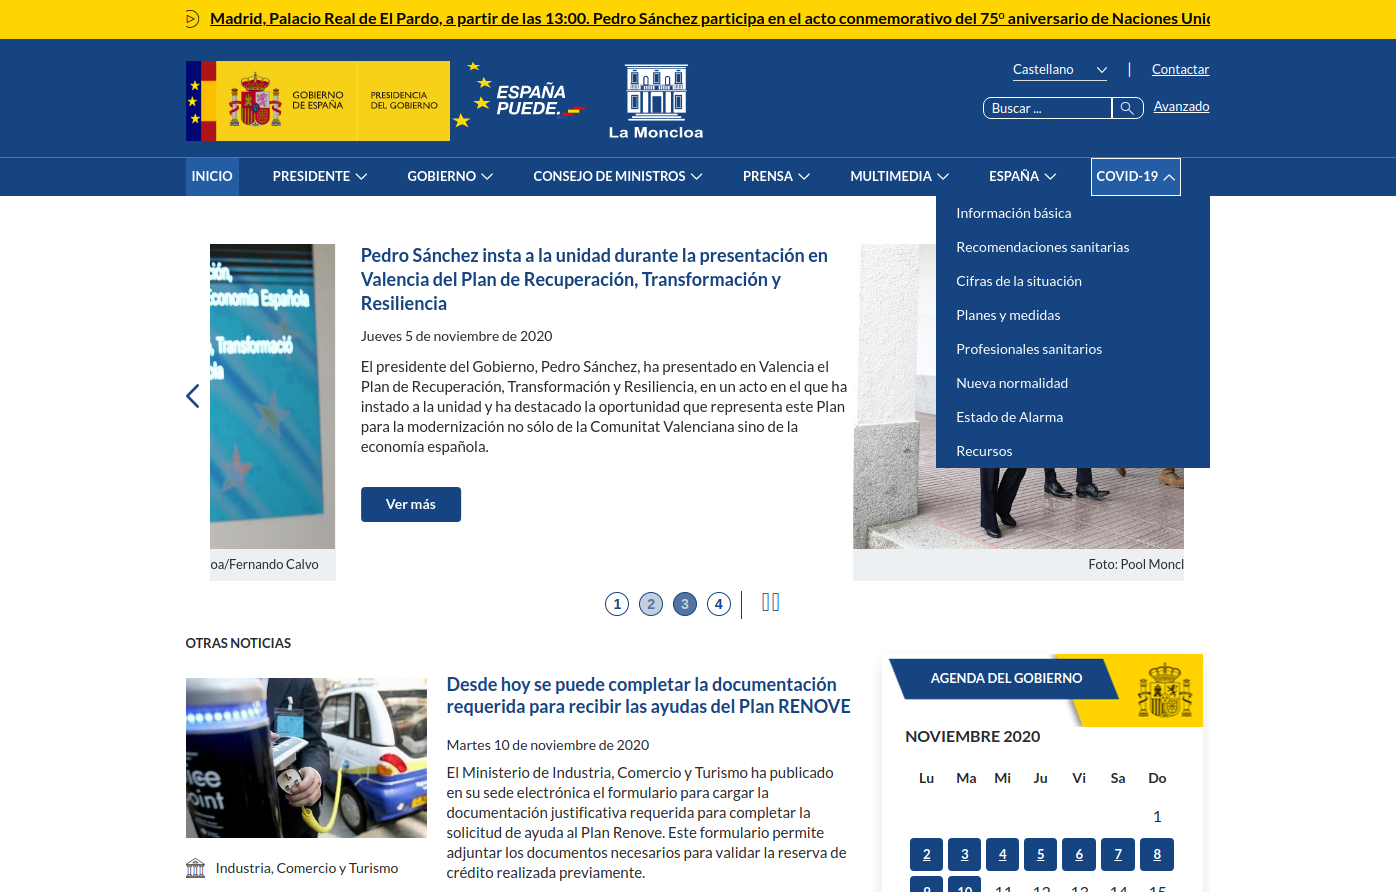
\includegraphics[width=1\textwidth]{img/inicio-moncloa}
	\caption{Página de inicio La Moncloa.}
	\label{fig:inicio-moncloa}
\end{figure}

\newpage
Una vez se ha redirigido al usuario, se le dará la opción de consultar los datos de España o los datos globales, junto con la opción de visualizar un video del proceso de recogida los datos en España, como se muestra en la Figura \ref{fig:opciones-moncloa}. Para este caso, la opción sobre la que nos centraremos es concretamente la que nos permite acceder a los datos a nivel de España, el usuario la seleccionará y será redirigido a una web del Ministerio de Sanidad \cite{gob-espana}, la cual vemos en la Figura \ref{fig:ministerio-salud}.

\begin{figure}[H]
	\centering
	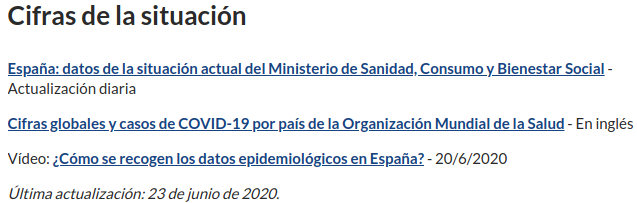
\includegraphics[width=1\textwidth]{img/opciones-moncloa}
	\caption{Opciones de consulta de La Moncloa.}
	\label{fig:opciones-moncloa}
\end{figure}

\begin{figure}[H]
	\centering
	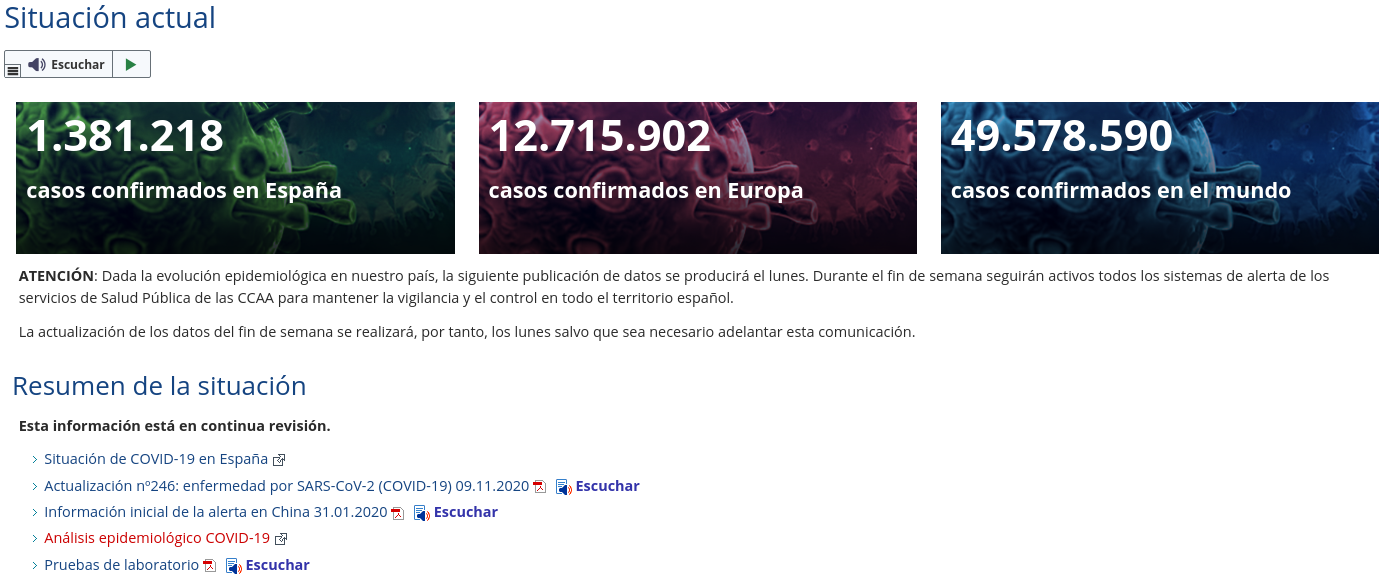
\includegraphics[width=1\textwidth]{img/ministerio-salud}
	\caption{Página de consulta del Covid-19 del Ministerio de Sanidad.}
	\label{fig:ministerio-salud}
\end{figure}

Dentro de la página del Ministerio de Sanidad lo primero que llama la atención y más resalta es el total de casos confirmados a nivel de España, de Europa y del Mundo. Además se indica al usuario que los datos, debido a la situación excepcional, se publicarán los lunes, de manera que la evolución de estos se verá semanalmente. Dentro de las opciones que se permiten seleccionar, el usuario tendrá seleccionar dos de ellas, en primer lugar \textit{Situación de COVID-19 en España}, la cual redirigirá al usuario a un mapa del territorio español interactivo donde lo único que se podrá consultar será la incidencia acumulada de las Comunidades Autónomas en los últimos 7 y 14 días como se muestra en la Figura \ref{fig:mapa-situacion}.

\begin{figure}[H]
	\centering
	\includegraphics[width=1\textwidth]{img/mapa-situación}
	\caption{Mapa con la incidencia acumulada por Comunidades Autónomas.}
	\label{fig:mapa-situacion}
\end{figure}

Otras de las opciones que el usuario puede seleccionar es la \textit{Actualización nº X}, que le permitirá visionar un pdf donde se encuentra toda la información unificada en tablas y posteriormente una serie de gráficas asociadas a las mismas. Dentro de toda la información que se nos proporciona, podemos ver la siguiente repartida en diversas tablas:

\begin{itemize}
	\item Casos de COVID-19 confirmados totales, diagnosticados el día previo y diagnosticados o con fecha de inicio de síntomas en los últimos 14 y 7 días.
	\item Casos de COVID-19 que han precisado hospitalización e ingreso en UCI. 
	\item Situación capacidad asistencial y actividad Covid-19 en hospitales.
	\item Total de Pruebas diagnósticas realizadas.
	\item Casos de COVID-19 que han fallecido (total y con fecha de fallecimiento en los últimos 7 días).
	\item Nº de casos COVID-19 importados de otro país.
	\item Detalles de los quince países con más casos confirmados de Europa
	\item Casos confirmados de COVID-19 fuera de Europa.
	\item Detalles de los quince países con más casos confirmados fuera de Europa
\end{itemize}

Si se quiere ver el modelo con el que se muestra esta información podemos acceder desde aquí \cite{actualizacion-gob}.

Como se ha podido de ver en el análisis, el acceso a los datos que nos proporciona el \textbf{Gobierno de España} es más o menos sencillo, pero para la gente que apenas usa esta web, mostrar un archivo pdf donde se representen enormes tablas con diversos datos que, aunque relacionados, cuando superan cierta cantidad pueden llegar a ser confusos, y gráficas separadas por varias páginas de estas tablas de datos, no es la mejor práctica posible.

\subsection{Comparativa}

Una vez hecho el análisis de la única opción conocida que puede llegar a aportar datos similares a los que queremos mostrar con nuestra aplicación, procederemos a hacer una comparativa con los diferentes requisitos que definimos con anterioridad.

Como hemos dicho antes, no compararemos los puntos 11-14 porque estos se han considerado que están asociados a un aplicación móvil y no a una página web como es el caso. En cuanto a los requisitos restantes, en referencia al 1, es cierto que podemos ver los datos de las diferentes Comunidades Autónomas, pero al tratarse de un simple documento pdf es imposible realizar una selección de las mismas.

En cuanto al resto de requisitos (2-9), todos ellos son visibles dentro del documento que nos proporciona la página web. En cuanto al requisito 10, queda claro, como se ha mencionado antes, que la visualización tanto de datos y gráficas no es ordenada y mucho menos clara, sobre todo cuando se acumulan varios tipos de información.

Es cierto que en la información proporcionada por el \textbf{Gobierno de España} es muy completa, como debe esperarse de la máxima autoridad del país, pero eso no hace que sea perfecta. La principal idea de la aplicación que se va a desarrollar es poder facilitar el acceso a estos datos al usuario, permitiendole acceder de manera sencilla e intuitiva a los mismos y seleccionar la información que desea utilizar. Es decir, lo que se pretende es una aplicación sencilla e interactiva, cosa que no se nos proporciona por parte del \textbf{Gobierno de España}.

\section{Recursos necesarios} \label{sec:recursos}

\subsection{Telegram}

\begin{figure}[H]
	\centering
	
\includegraphics[width=0.2\textwidth]{img/telegram-icon}
	\caption{Logotipo de Telegram.}
\end{figure}

\textbf{Covid-19 Reports} está concebido para ser un chatbot, por lo que la primera decisión que se ha tenido que tomar ha sido la plataforma donde se implementará. Hay muchas aplicaciones sobres las que se podría llevar a cabo el desarrollo de este chatbot, aunque para este punto se han considerado solo dos de ellas: WhatsApp \cite{whatsapp} y Telegram \cite{telegram}. En un artículo de la web Xataka Android \cite{articulo-xataka}, se lleva a cabo una explicación punto por punto de las diferencias entre ambas aplicaciones finalizando con una tabla que mostramos en la Figura \ref{fig:tabla-comparativa}

\begin{figure}[H]
	\centering
	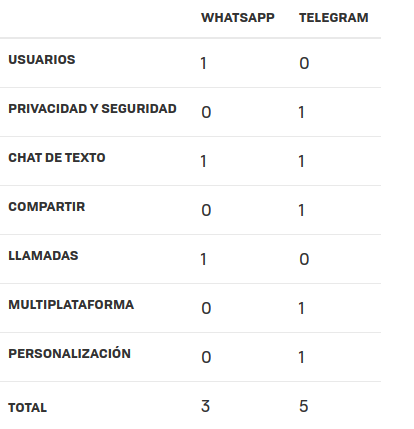
\includegraphics[width=0.6\textwidth]{img/tabla-comparativa}
	\caption{Tabla comparativa WhatsApp vs Telegram. Fuente: Xataka \cite{articulo-xataka}}
	\label{fig:tabla-comparativa}
\end{figure}

Existen varias razones por las que se ha optado por hacer uso de \textbf{Telegram}, entre ellas podemos destacar las siguientes:

\begin{enumerate}
	\item \textbf{Contenido disponible a través de Bots:} en el caso de \textbf{Telegram}, la lista de contenidos se ve multiplicada gracias a estos. Es cierto que \textbf{WhatsApp} también puede permitir la implementación de Bots, pero aún no es algo que se pueda realizar de manera generalizada, mientras que en \textbf{Telegram} cualquier usuario puede crear sus propios Bots.
	\item \textbf{Cuentas asociadas a un nº de teléfono:} \textbf{WhatsApp} tiene sus cuentas de usuario enlazadas a los números de teléfono de los usuarios, lo que implica que no se puede chatear con alguien sin tener su nº de teléfono. Sin embargo, \textbf{Telegram} facilita la comunicación entre usuarios asignándole nombres de usuarios a los mismos. Esto implica un importante punto a favor de \textbf{Telegram} en el ámbito de la privacidad, ya que en \textbf{WhatsApp} mientras formemos parte de un grupo todos los usuarios que se encuentre en este pueden ver nuestro nº de teléfono, \textbf{Telegram} mostrará en su lugar el nombre de usuario, impidiendo al resto conocer nuestro nº de teléfono.
	\item \textbf{Versión Web:} En este punto \textbf{Telegram} es el claro ganador. Aunque las dos aplicaciones cuentan con una versión Web, \textbf{WhatsApp} presenta un gran defecto que no se puede dejar pasar, y más a la hora de desarrollar una aplicación como esta: la estricta necesitad de tener el dispositivo móvil activo y conectado a Internet. En este aspecto, \textbf{Telegram} presenta una independencia total entre la versión de dispositivos y Web.
	\item \textbf{Descargas de contenido:} Sabiendo que queremos mostrar diferentes imágenes para favorecer el entendimiento de los datos a los usuarios, el evitar llenar la memoria de sus dispositivos es algo muy importante. \textbf{Telegram} almacena estos contenidos en la nube, por lo que no será necesario descargarlos para poder visionarlos, mientras que en \textbf{WhatsApp} por el contrario si queremos visualizar este contenido, tendríamos que permitir su almacenamiento en la memoria del dispositivo.
\end{enumerate}

\subsection{Python}

\begin{figure}[H]
	\centering
	
\includegraphics[width=0.2\textwidth]{img/python-icon}
	\caption{Logotipo de Python.}
\end{figure}

Como lenguaje de programación se ha optado por elegir \textbf{Python}. En primer lugar se debe a que es un lenguaje sobre el que he trabajado en varias ocasiones y es uno de los lenguajes más fáciles de manejar. Otra de las razones por las que he decidido trabajar en \textbf{Python} se debe a que a la hora de analizar datos y poder representarlos de manera gráfica, acciones que he podido probar en diversos lenguajes de programación y que \textbf{Python} permite realizar de manera más sencilla. Y no solo por ello, si no también por su popularidad. Según un artículo de Stackscale \cite{articulo-stackscale}, \textbf{Python} se ha convertido en el más utilizado, llegando a superar a \textbf{Java}, en los rankings de GitHub en 2019.

No solo por ello, se ha tenido en cuenta las características del proyecto y con que se va a trabajar. No solo es importante la interfaz del Bot, también lo es el contexto en el que trabajará, siendo en este caso el análisis de datos. Teniendo esto, aparece un nuevo lenguaje de uso común para el análisis de datos, \textbf{R}. Pero, ¿por que escogeremos a \textbf{Python} como el lenguaje principal de nuestro proyecto?

Según Paula Rochina en su artículo \cite{articulo-revista-digital} estas son las principales causas por las que debemos decantarnos por \textbf{Python}:

\begin{enumerate}
	\item \textbf{Python} es un lenguaje dinámico, lo que quiere implica que podremos cambiar el tipo de una variable o agregar nuevas propiedades o métodos a un objeto mientras el programa está en ejecución.
	\item La curva de aprendizaje de \textbf{Python} no es muy exigente, es un lenguaje sencillo de aprender tanto para nuevos programadores como para programadores que quieren incrementar las habilidades que tienen del mismo.
	\item Dado que el análisis de datos que se lleva a cabo en el proyecto no es independiente al mismo, si no que ha de estar integrado en nuestro Bot, \textbf{Python} es la mejor opción frente a \textbf{R}
\end{enumerate}

Para una mayor seguridad a la hora de elegir este lenguaje mencionaremos a artículo de Planeta CHATBOT, escrito por Marvin G. Soto \cite{articulo-planeta-chatbot} donde, como resumen, \textbf{Python} es la mejor alternativa para un chatbot al admitir todo tipo de funcionalidades y garantiza un acceso rápido y fácil a la información y los servicios de la aplicación como usuarios.

Una vez decidido sobre que lenguaje se va a desarrollar el proyecto explicaremos las diferentes librerías o paquetes que van a ser necesarios para poder desarrollar el Bot: python-telegram-bot, pandas y Matplotlib.

\subsubsection{python-telegram-bot}

\begin{figure}[H]
	\centering
	
\includegraphics[width=0.5\textwidth]{img/python-telegram-bot-icon}
	\caption{Logotipo de python-telegram-bot.}
\end{figure}

Se ha decidido escoger esta librería ya que proporciona al usuario una interfaz Python pura para el \textbf{Telegram Bot API}. Además de que es una librería que se actualiza con regularidad, ésta es compatible con las versiones más actuales de \textbf{Python}, siendo éstas las superiores a su versión 3.6. Además la biblioteca cuenta con algunas funciones para facilitar el desarrollo de Bots, haciéndolo mas fácil y sencillo.

Para mas información puede consultarse su repositorio en GitHub \cite{python-telegram-bot}

\subsubsection{pandas}

\begin{figure}[H]
	\centering
	
\includegraphics[width=0.2\textwidth]{img/pandas-icon}
	\caption{Logotipo de pandas.}
\end{figure}

la librería \textbf{pandas}, se considera una extensión de NumPy para poder manipular y analizar datos en \textbf{Python}. Se ha decidido utilizarla ya que previamente he trabajado con ella para aplicarla en ámbitos de Machine Learning, además en éste caso porque nos permite leer de manera fácil archivos de formato CSV (explicaremos más adelante porque hacemos uso de éstos archivos). También nos permite de una manera sencilla poder trabajar con tablas, acceder a sus índices, reordenarlas, modificarlas y combinarlas.

Para más información puede consultarse desde su web \cite{pandas}

\subsubsection{matplorlib}

\begin{figure}[H]
	\centering
	
\includegraphics[width=0.4\textwidth]{img/matplotlib-icon}
	\caption{Logotipo de Matplotlib.}
\end{figure}

\textbf{Matplotlib} es una librería de \textbf{Python} dedicada a la generación de gráficos por medio de datos. Ésta combina a la perfección con \textbf{pandas}. Durante principios de 2020 he tenido la oportunidad de trabajar con diferentes bibliotecas gráficas para \textbf{Python}, como Sklearn. Al trabajar con ambas al mismo tiempo me llegué a sentir mas cómodo con \textbf{Matplotlib}, ya que me parecía más sencilla de utilizar. Por ello se ha optado por su uso para este proyecto.

Para más información puede consultarse desde su web \cite{matplotlib}

\subsection{Git y GitHub}

\begin{figure}[H]
	\centering
	
\includegraphics[width=0.4\textwidth]{img/git-icon}
	\caption{Logotipo de Git.}
\end{figure}

\textbf{Git} es un software de control de versiones. Está pensado para la eficiencia y la confiablilidad del mantenimiento entre versiones de aplicaciones cuando éstas tienen un gran número de archivos de código fuente. \textbf{Git} nace de la necesidad de llevar un control de los cambios de los archivos y sobre el trabajo que diferentes personas puedan realizar sobre archivos que se encuentran compartidos en un proyecto.

\begin{figure}[H]
	\centering
	
\includegraphics[width=0.2\textwidth]{img/github-icon}
	\caption{Logotipo de GitHub.}
\end{figure}

\textbf{GitHub} es una plataforma que nos permite alojar proyectos haciendo uso del \textbf{Git}. Se ha decidido utilizar esta plataforma para alojar nuestro código ya que se pretende que sea un proyecto de software libre haciendo uso de una licencia \textbf{AGPL} \cite{agplv3}.

\subsection{Heroku}

\begin{figure}[H]
	\centering
	
\includegraphics[width=0.3\textwidth]{img/heroku-icon}
	\caption{Logotipo de Heroku.}
\end{figure}

Partiendo del punto en el que al crear un Bot para \textbf{Telegram} se obtienen unos TOKENS que son necesarios y están asociados al Bot en la aplicación y al ser un TOKEN que otorga manejo total sobre nuestro Bot no debe ser mostrado en ningún momento. Desde \textbf{Heroku} podremos proteger este TOKEN, permitiendo guardarlo con una variable de configuración, donde solo el dueño de la aplicación puede tener acceso a ellos y no son visibles en el código. \textbf{Heroku} es un PaaS (Platform as a Service) que nos permitirá poder desplegar nuestro Bot en la nube de manera que siempre esté en funcionamiento y podamos hacer uso de él en todo momento.

Para más información puede consultarse desde su web \cite{heroku}

A lo largo de este capítulo se ha podido observar y analizar los puntos importantes del arte de nuestro proyecto, comparando con otras aplicaciones o webs que pueden asimilarse a lo que se quiere llevar a cabo, así como las principales herramientas que se van a utilizar para desarrollar el mismo.

	% Desarrollo bajo sprints: 
	% 	1. Permitir registros y login de usuarios
	% 	2. Desarrollo del sistema de incidencias
	% 	3. Desarrollo del sistema de denuncias administrativas y accidentes
	% 	4. Desarrollo del sistema de croquis
	%   5. Instalación de la aplicación de manera automática
	\chapter{Planificación} \label{ch:planificación}

\section{Metodología utilizada}

Para poder planificar este proyecto se ha optado por hacer uso de una de las metodologías ágiles mas utilizadas hoy en día, la metodología Scrum. Scrum es una metodología ágil para el desarrollo de software la gestión de proyectos. Antes de centrarnos en definir en que consiste aplicar una metodología Scrum es muy importante conocer que es una metodología ágil.

\subsection{Metodología Ágil}

La metodología ágil, más que una forma para llevar a cabo proyectos que requieren de rapidez y flexibilidad podría llegar a concebirse como una filosofía que presenta una forma distinta de trabajar y organizarse, adaptándose a las condiciones cambiantes que pueden surgir, aprovechando los cambios para obtener ventajas. Por medio de esta lo que se pretende es dividir un proyecto en pequeñas partes, de manera que este se realice de forma incremental o por fases, permitiendo así que dichas partes se pueden completar y entregarse lo mas rápido posible. 

Es importante tener en cuenta al definir la metodología ágil el propio manifiesto ágil \cite{manifiesto-agil}, que contiene los valores sobre los que se asientan dichos métodos y fuéron definidos en 2001. Estos valores son los siguientes:

\begin{itemize}
	\item Individuos e interacciones sobre procesos y herramientas
	\item Software funcionando sobre documentación extensiva
	\item Colaboración con el cliente sobre negociación contractual
	\item Respuesta ante el cambio sobre seguir un plan
\end{itemize}

Llevar a cabo una implementación ágil consta de 2 fases: análisis y realización de Sprint como se muestra en la Figura \ref{fig:metodologia-agil}.

\begin{figure}[h]
	\centering
	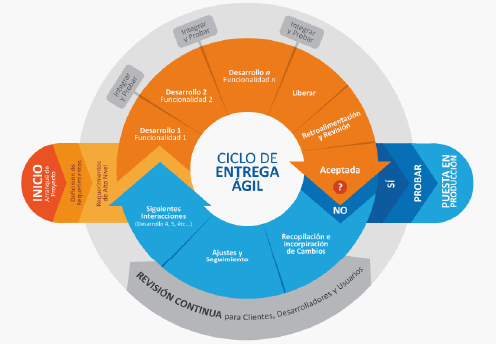
\includegraphics[width=1\textwidth]{img/metodologia-agil}
	\caption{Ciclo de entrega en proyectos ágiles.}
	\label{fig:metodologia-agil}
\end{figure}

A continución veremos en que consisten ambas fases:

\subsubsection{Fase 1: Análisis} \label{sssec:fase-analisis}
Esta fase consiste en 4 pasos:
\begin{enumerate}
	\item Preparación del proyecto durante el cual se definen los diferentes elementos, tales como labores,responsabilidades, estándares para la documentación y requisitos del hardware.
	\item Proceso de visualización en el que se identifican cuidadosamente todos los procesos operativos y procesos que dependen de condiciones específicas, como seguridad, autorizaciones e interfaces. Estos resultados serán la base para la construcción de unos cimientos sólidos para el proyecto entero.
	\item Funcionamiento de referencia del sistema, el cual se basará en el software de ERP.
	\item Fase de evaluación. En esta fase, se determina la prioridad de los requisitos adicionales y las funcionalidades, en orden del valor del negocio. Después de esto, el equipo de implementación estima el esfuerzo que será necesario para realizar esto y determina la planificación de los Sprints para que se suministren los componentes del sistema.
\end{enumerate}

\subsubsection{Fase 2: Realización del Sprint}

Esta fase consiste en 5 pasos:

\begin{enumerate}
	\item Reuniones de planificación al comienzo de cada Sprint. Se define el objetivo del Sprint entre el propietario y el equipo de implementación.
	\item Realización de los requisitos, de pruebas y documentación.
	\item Reuniones diarias del estado del proyecto. En esta fase se registra el estado del proyecto y se discuten los diversos obstáculos que el equipo ha podido encontrar.
	\item Sesión de prueba del Sprint. Durante esta fase los usuarios y el equipo IT determinan si los procesos cumplen los requisitos.
	\item Se llevará a cabo una revisión del Sprint para comprobar que se puede mejorar en los futuros Sprints.
\end{enumerate}

\subsection{Metodología Scrum}

Como hemos dicho al inicio de este capítulo, Scrum es una metodología ágil para el desarrollo de software o la gestión de proyectos, más específicamente, es un marco de trabajo a través del cual las personas pueden abordar problemas complejos adaptativos, mientras que se entregan productos de forma eficiente y creativa con el máximo valor \cite{scrum-guia}.

Scrum está compuesto por diferentes procesos que se utilizan para la gestión del trabajo de producto complejos desde inicios de los años 90. Como tal, Scrum no es un proceso, una técnica o un método definitivo, es un marco de trabajo donde se puede emplear un conjunto de diversos procesos o técnicas. Scrum muestra la eficacia relativa de las técnicas de gestión de producto y de trabajo de modo que podamos mejorar de forma continua el producto, equipo y entorno de trabajo. El marco de trabajo de Scrum está compuesto por los Equipos Scrum, sus Roles, Eventos, Artefactos y Reglas asociadas. Cada uno de ellos sirve a un propósito específico y de la misma forma es esencial para el éxito de Scrum y para su uso.

En un principio, Scrum fue desarrollado para gestionar y desarrollar productos. Con el tiempo, y más a partir de 1990, se ha llegado a utilizar en diferentes ámbitos: desarrollo de software, hardware, redes funcionales, vehículos autónomos, escuelas, gobiernos, marketing y en la totalidad de todo lo que hacemos uso en nuestra vida, tanto como individuos y sociedad.

La esencia de Scrum reside en trabajar en pequeños equipos, siendo estos individualmente flexibles y adaptativos. Estas características siguen manteniéndose tanto en equipos individuales, varios, muchos u redes que equipos encargados de desarrollar, lanzar, operar y mantener el trabajo y el producto. Entre los diferentes equipos colaboran e ínter-operan a través del desarrollo de sofisticadas arquitecturas y objetivos en entornos de desarrollo.

\subsubsection{Características de Scrum}

Entre todas las metodologías ágiles, Scrum se basa en la teoría de control empírica de los procesos. Esto significa que se utiliza el progreso real de un proceso para poder planificar y concretar los lanzamientos. Scrum trabaja de forma que los proyectos están divididos en Sprints, los cuales tienen una duración de entre dos a cuatro semanas. Cuando finaliza un Sprint, se realiza una reunión entres los miembros del equipo y el cliente con el fin de mostrar al cliente el proyecto y que este pueda ser evaluado de cara a poder planificar las tareas que se deberán de utilizar en el siguiente Sprint como se ve en la Figura \ref{fig:scrum}. Con esto lo que se pretende es que la dirección del proyecto pueda ajustarse o reorientarse una vez haya finalizado y durante el mismo mantener un control de los riesgos.

\begin{figure}[h]
	\centering
	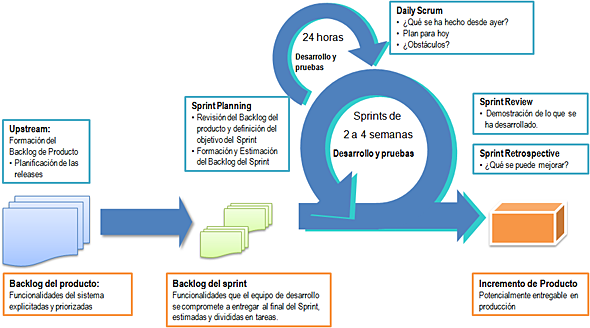
\includegraphics[width=1\textwidth]{img/scrum}
	\caption{Ciclo de vida de Scrum.}
	\label{fig:scrum}
\end{figure}

\newpage
Existen tres pilares sobre los que se fundamentará el control empírico de Scrum:

\begin{enumerate}
	\item \textbf{Transparencia:} Los aspectos significativos han de ser visibles para todos aquellos responsables del resultado.
	\item \textbf{Inspección:} Se han de inspeccionar frecuentemente los artefactos y el progreso hacia el objetivo, para detectar variaciones.
	\item \textbf{Adaptación:}  Capacidad para adaptarse en el caso de que el procesose desvíe de los límites aceptables.
\end{enumerate}

\subsubsection{Roles de Scrum}

Un equipo de \textbf{Scrum} suele estar formados por unos pocos miembros, entre 3 y 9, sin incluir al Scrum Manager y el Product Owner. Cada uno de ellos tiene por tanto diferentes roles y responsabilidades dentro del proyecto. Procederemos a continuación a explicar las diferentes responsabilidades de cada uno de ellos

\begin{itemize}
	\item \textbf{Product Owner}: Es el rol principal del proyecto. Suele ser el encargado de representar al cliente o ser directamente el propio cliente. ha de preservar los intereses del cliente priorizando las diferentes tareas para alcanzar los objetivos propuestos y establecer los diferentes requisitos del proyecto. De los tres roles, es el que mayor responsabilidades tiene, por lo que si algo no funciona o sale mal la responsabilidad recae sobre el. Para que el Product Owner pueda hacer bien su trabajo, todos han de respetar sus decisiones. A su vez el Product Owner debería evitar la supervisión de cada detalle del proyecto, pero sin embargo ha de estar disponible en caso de que el equipo de desarrollo tenga alguna pregunta o duda.
	\item \textbf{Scrum Master}: Es el rol encargado de actuar como enlace entre el Product Owner y el equipo de desarrollo. Como tal el Scrum Master ha de encargarse de resolver los diferentes conflictos que puedan obstaculizar el ritmo del proyecto. Este a su vez ha de incentivar u motivar al equipo de desarrollo para poder hacer visibles los logros del mismo ante del Product Owner. De cara al Product Owner, el Scrum Master le ofrecerá el apoyo necesario para poder maximizar los resultados.
	\item \textbf{Equipo de desarrollo}: Es el rol que se le da al conjunto del equipo que trabaja en el equipo, el cual será el encargado de terminar el trabajo. Estos equipos han de ser auto-organizados, multifuncionales, aunque cada miembro del equipo puede tener habilidades especializadas en un área, aunque la responsabilidad recae sobre el equipo y no sobre el individuo. A su vez, no se reconocen títulos dentro del equipo, independientemente del trabajo que realicen sus mienbros así como tampoco se reconocen  los sub-equipo, independientemente de los dominios sobre lso que se trabajen
\end{itemize}

\begin{figure}[H]
	\centering
	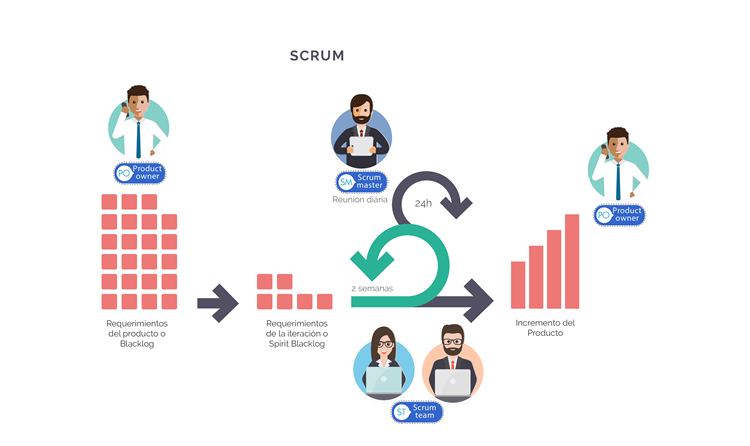
\includegraphics[width=1\textwidth]{img/roles-scrum}
	\caption{Estructura de la participación de los roles en el Scrum.}
	\label{fig:roles-scrum}
\end{figure}

\section{Historias de usuario y tareas} \label{sec:historias-tareas}

En este punto se tiene que ser capaz de plantear los objetivos que han de ser alcanzados a lo largo del desarrollo del producto final. Para hacer esto se hará uso de una serie de \textbf{Historias de Usuarios}, un elemento básico a la hora de aplicar metodologías ágiles en un proyecto y especialmente para poder aplicar \textbf{Scrum}. Las \textbf{Historias de Usuario} representarán de manera breve las características demandadas por el cliente las cuales deberán formar parte de la funcionalidad del producto, satisfaciendo sus exigencias.

El proceso por el cual se realiza la extracción de información relacionada con la funcionalidad del proyecto se debe llevar a cabo entre los miembros del equipo y el propio cliente. Al aplicar \textbf{Scrum}, este proceso no solo se realizará en la fase inicial del proyecto, si no que se realizan en cada Sprint del proyecto, de manera que se pueda obtener el resultado esperado en un corto espacio de tiempo y permitiendo amoldar el proyecto a lo requerido por el cliente de la forma mas eficiente posible.

Las \textbf{Historias de Usuario}, en términos generales, siempre han de extraerse durante las reuniones con el cliente y es deseable que sean escritas por el mismo y en un lenguaje claro, sin entrar en detalles. Estas han de aportarnos la funcionalidad requerida por el proyecto, entregando de esta forma un valor particular al cliente.

Estas han de desglosarse en tres apartados:

\begin{itemize}
	\item \textbf{Como}: representa el rol que va a utilizar el proyecto
	\item \textbf{Quiere}: representa la acción o evento que quiere que ocurra
	\item \textbf{Para}: representa la funcionalidad que se quiere cubrir.
\end{itemize}

A su vez tambien puede usarse la estructura presentada por la web Scrum Manager \cite{scrum-manager}:

\begin{itemize}
	\item Nombre breve y descriptivo.
	\item Descripción de la funcionalidad en forma de diálogo o monólogo del usuario describiendo la funcionalidad que desea realizar.
	\item Criterio de validación y verificación que determinará para considerar terminado y aceptable por el cliente el desarrollo de la funcionalidad descrita.
\end{itemize}

Como se ha dicho antes, las \textbf{Historias de Usuario} ayudan a modelar el producto según las necesidades del cliente y mediante una reunión entre el equipo y este. El cliente aportará la idea que tiene, las necesidades que pretende cubrir y las funcionalidades que en cada momento el estima oportunas para el proyecto. A su vez, el equipo encargado del desarrollo también podrán aportar su punto de vista en ciertos puntos con la finalidad de poder enriquecer el proyecto. Para finalizar el Product Owner, que actúa como la voz del cliente dentro del equipo, será el encargado de redactar las \textbf{Historias de Usuario} y de extraer las diferentes tareas resultantes de las mismas, identificandolas según el coste su coste y prioridad. Con esto lo que se consigue es definir el Product Backlog, base a la hora de aplicar Scrum a un proyecto.

Es importante recalcar que en el Product Backlog se indicaran los diferentes Sprints del proyecto y las tareas asociadas a los mismos. Esto no quiere decir que se mantenga durante todo el proyecto, pues la definición obtenida al inicio del mismo puede varias dependiendo de las necesidades del cliente. Dado que el proyecto estará dividido en una serie de Sprints, durante los mismos debería realizarse una reunión entre los diferentes miembros del equipo y el cliente donde se podrán hacer adaptaciones que se consideren convenientes permitiendo cambiar o replantear los objetivos del proyecto con el fin de maximizar su utilidad.

Las \textbf{Historias de Usuario} serán definidas con la siguiente estructura:

\rowcolors{1}{gray!30}{gray!10}
\begin{table}[H]
	\begin{center}
		\begin{tabular}{| c | p{9cm} |}
			\hline
			
			Historia de Usuario &  \\ \hline
			
			
			\textbf{ID} & HUXX \\
			\textbf{Nombre} &  \\
			\textbf{Prioridad} &  \\
			\textbf{Riesgo} &  \\
			\textbf{Descripción} &  \\
			\textbf{Validación} &  \\ \hline
		\end{tabular}
		\caption{Modelo Historia de Usuario.}
	\end{center}
\end{table}

Cada campo de las \textbf{Historias de Usuario} representa lo siguiente:

\begin{itemize}
	\item \textbf{ID}: Identificar único de la Historia de Usuario.
	\item \textbf{Nombre}: Nombre asignado a la Historia de Usuario
	\item \textbf{Prioridad}: Importancia a la hora de llevar a cabo en el desarrollo, pudiendo ser alta, media o baja
	\item \textbf{Riesgo}: Importancia en relación al conjunto del proyecto, indicando así en caso de fallo el daño provocado, pudiendo ser alto, medio o bajo. .
	\item \textbf{Descripción}: Explicación de la Historia de Usuario, dejando clara la idea de la misma
	\item \textbf{Validación}: Condiciones que se han de cumplir para dar la historia por finalizada.
\end{itemize}

\subsection{Historias de Usuario}

Las \textbf{Historias de Usuario} que se han creado para este proyecto son las siguientes:

\rowcolors{1}{gray!30}{gray!10}
\begin{table}[H]
	\begin{center}
		\begin{tabular}{| c | p{9cm} |}
			\hline
			
			Historia de Usuario &  \\ \hline
			
			
			\textbf{ID} & HU01 \\
			\textbf{Nombre} & Apariencia \\
			\textbf{Prioridad} & Media \\
			\textbf{Riesgo} & Baja \\
			\textbf{Descripción} & Como usuario quiero que el bot tenga un diseño simple, sencillo e intuitivo. \\
			\textbf{Validación} & \begin{itemize}
				\item Quiero acceder a la información pulsando un botón.
				\item Quiero ver todos los datos de manera clara.
				\item Todos los botones han de tener un funcionamiento claro.
			\end{itemize} \\ \hline
		\end{tabular}
		\caption{Historia de Usuario - Apariencia.}
	\end{center}
\end{table}

\begin{table}[H]
	\begin{center}
		\begin{tabular}{| c | p{9cm} |}
			\hline
			
			Historia de Usuario &  \\ \hline
			
			
			\textbf{ID} & HU02 \\
			\textbf{Nombre} & Funcionamiento \\
			\textbf{Prioridad} & Media \\
			\textbf{Riesgo} & Baja \\
			\textbf{Descripción} & Como usuario quiero poder hacer uso del Bot en todo momento, principalmente en un dispositivo móvil, para poder consultar información en cualquier lugar. \\
			\textbf{Validación} & \begin{itemize}
				\item Quiero que el Bot funcione sobre todo en móviles.
				\item Quiero que tenga un acceso fácil.
			\end{itemize} \\ \hline
		\end{tabular}
		\caption{Historia de Usuario - Funcionamiento.}
	\end{center}
\end{table}

\begin{table}[H]
	\begin{center}
		\begin{tabular}{| c | p{9cm} |}
			\hline
			
			Historia de Usuario &  \\ \hline
			
			
			\textbf{ID} & HU03 \\
			\textbf{Nombre} & Menú Principal \\
			\textbf{Prioridad} & Alta \\
			\textbf{Riesgo} & Baja \\
			\textbf{Descripción} & Como usuario quiero tener un menú principal que se muestre en todo momento y me permita acceder a las diferentes utilidades del Bot. \\
			\textbf{Validación} & \begin{itemize}
				\item Quiero que el menú se muestre siempre por defecto salvo que el usuario decida ocultarlo.
				\item Quiero poder acceder al menú principal del Bot.
				\item Quiero poder acceder a la ayuda del Bot.
				\item Quiero poder acceder a la información de desarrollo del Bot.
			\end{itemize} \\ \hline
		\end{tabular}
		\caption{Historia de Usuario - Menú Principal.}
	\end{center}
\end{table}

\begin{table}[H]
	\begin{center}
		\begin{tabular}{| c | p{9cm} |}
			\hline
			
			Historia de Usuario &  \\ \hline
			
			
			\textbf{ID} & HU04 \\
			\textbf{Nombre} & Seleccionar Comunidad Autónoma \\
			\textbf{Prioridad} & Alta \\
			\textbf{Riesgo} & Baja \\
			\textbf{Descripción} & Como usuario quiero poder seccionar la provincia de la que quiero consultar los datos. \\
			\textbf{Validación} & \begin{itemize}
				\item Quiero poder seleccionar entre todas las CCAA del territorio español.
				\item Quiero poder seleccionar toda España.
				\item Las CCAA deben verse todas a la vez en pantalla.
				\item Las CCAA han de mostrarse de manera clara y ordenada.
			\end{itemize} \\ \hline
		\end{tabular}
		\caption{Historia de Usuario - Selección Comunidad Autónoma.}
	\end{center}
\end{table}

\begin{table}[H]
	\begin{center}
		\begin{tabular}{| c | p{9cm} |}
			\hline
			
			Historia de Usuario &  \\ \hline
			
			
			\textbf{ID} & HU05 \\
			\textbf{Nombre} & Seleccionar datos \\
			\textbf{Prioridad} & Alta \\
			\textbf{Riesgo} & Media \\
			\textbf{Descripción} & Como usuario quiero poder seccionar los datos que quiero consultar. \\
			\textbf{Validación} & \begin{itemize}
				\item Los datos han de mostrarse en diferentes apartados.
				\item Pueden consultarse los datos mas actuales.
				\item Pueden consultase los datos desde el inicio de la pandemia.
				\item En algunos datos deben mostrarse gráficas (mostrar evolución de manera clara).
				\item Poder consultar la acumulación de casos.
				\item Poder ver el nº de fallecidos.
				\item Poder ver el nº de hospitalizados.
				\item Poder ver una lista de las provincias con más casos (solo al consultar España)
				\item Poder ver las incidencias actuales por cada 100k habitantes por provincias (solo al consultar España)
				\item Poder ver las incidencias desde el inicio de la pandemia por cada 100k habitantes por provincias (solo al consultar España)
				\item Poder ver como afecta el virus dependiendo de la edad (solo al consultar España)
			\end{itemize} \\ \hline
		\end{tabular}
		\caption{Historia de Usuario - Selección datos.}
	\end{center}
\end{table}

\begin{table}[H]
	\begin{center}
		\begin{tabular}{| c | p{9cm} |}
			\hline
			
			Historia de Usuario &  \\ \hline
			
			
			\textbf{ID} & HU06 \\
			\textbf{Nombre} & Seleccionar ayuda \\
			\textbf{Prioridad} & Alta \\
			\textbf{Riesgo} & Baja \\
			\textbf{Descripción} & Como usuario quiero poder acceder a una opción en todo momento por si tengo alguna duda. \\
			\textbf{Validación} & \begin{itemize}
				\item Esta opción ha de mostrarse en todo momento salvo que el usuario la oculte.
				\item Esta opción ha de estar en el menú principal.
				\item Quiero poder ver que es cada uno de los apartados del proyecto.
			\end{itemize} \\ \hline
		\end{tabular}
		\caption{Historia de Usuario - Selección ayuda.}
	\end{center}
\end{table}

\begin{table}[H]
	\begin{center}
		\begin{tabular}{| c | p{9cm} |}
			\hline
			
			Historia de Usuario &  \\ \hline
			
			
			\textbf{ID} & HU07 \\
			\textbf{Nombre} & Seleccionar información \\
			\textbf{Prioridad} & Alta \\
			\textbf{Riesgo} & Baja \\
			\textbf{Descripción} & Como desarrollador quiero que el usuario pueda consultar datos sobre el proyecto. \\
			\textbf{Validación} & \begin{itemize}
				\item Esta opción ha de mostrarse en todo momento salvo que el usuario la oculte.
				\item Esta opción ha de estar en el menú principal.
				\item Quiero mostrar al usuario la información principal del desarrollo del proyecto.
			\end{itemize} \\ \hline
		\end{tabular}
		\caption{Historia de Usuario - Selección información.}
	\end{center}
\end{table}

\begin{table}[H]
	\begin{center}
		\begin{tabular}{| c | p{9cm} |}
			\hline
			
			Historia de Usuario &  \\ \hline
			
			
			\textbf{ID} & HU08 \\
			\textbf{Nombre} & Despliegue \\
			\textbf{Prioridad} & Alta \\
			\textbf{Riesgo} & Baja \\
			\textbf{Descripción} & Como desarrollador quiero que el Bot funcione en todo momento. \\
			\textbf{Validación} & \begin{itemize}
				\item El Bot y sus datos han de estar en un contenedor.
				\item El Bot ha de desplegarse como un PaaS.
			\end{itemize} \\ \hline
		\end{tabular}
		\caption{Historia de Usuario - Despliegue.}
	\end{center}
\end{table}

\begin{table}[H]
	\begin{center}
		\begin{tabular}{| c | p{9cm} |}
			\hline
			
			Historia de Usuario &  \\ \hline
			
			
			\textbf{ID} & HU09 \\
			\textbf{Nombre} & Modularización \\
			\textbf{Prioridad} & Alta \\
			\textbf{Riesgo} & Baja \\
			\textbf{Descripción} & Como programador, quiero modularizar algunas partes de forma que sean fáciles de manejar y testear. \\
			\textbf{Validación} & \begin{itemize}
				\item Quiero de los diferentes módulos puedan pasar los test.
				\item Quiero que el código esté dividido por funcionalidad.
			\end{itemize} \\ \hline
		\end{tabular}
		\caption{Historia de Usuario - Modularización.}
	\end{center}
\end{table}

\newpage
\subsection{Tareas}

A su vez, las \textbf{Historias de Usuario} estarán divididos en una serie de \textbf{Tareas}. Las \textbf{Tareas} serán definidas con la siguiente estructura:

\begin{table}[H]
	\begin{center}
		\begin{tabular}{| c | p{9cm} |}
			\hline
			
			\textbf{Tarea} & TXX \\
			\textbf{Historia de Usuario} &  \\
			\textbf{Estado} &  \\
			\textbf{Descripción} &  \\ \hline
		\end{tabular}
		\caption{Modelo Tarea.}
	\end{center}
\end{table}

Cada campo de las \textbf{Historias de Usuario} representa lo siguiente:

\begin{itemize}
	\item \textbf{Tarea}: Identificar único de la Tarea.
	\item \textbf{Historia de Usuario}: Historia de Usuario a la que está asociada la Tarea
	\item \textbf{Estado}: Fase en la que se encuentra la Tarea dentro del proyecto, pudiendo ser No iniciada, En proceso o Completada
	\item \textbf{Descripción}: Explicación de la Historia de Usuario, dejando clara la idea de la misma
\end{itemize}

Las \textbf{Tareas} que se han creado para este proyecto son las siguientes:

\begin{table}[H]
	\begin{center}
		\begin{tabular}{| c | p{9cm} |}
			\hline
			
			\textbf{Tarea} & T01 \\
			\textbf{Historia de Usuario} & HU02 \\
			\textbf{Estado} & Completada \\
			\textbf{Descripción} & Seleccionar la plataforma donde vamos a desarrollar el Bot \\ \hline
		\end{tabular}
		\caption{Tarea 01.}
	\end{center}
\end{table}

\begin{table}[H]
	\begin{center}
		\begin{tabular}{| c | p{9cm} |}
			\hline
			
			\textbf{Tarea} & T02 \\
			\textbf{Historia de Usuario} & HU01 \\
			\textbf{Estado} & Completada \\
			\textbf{Descripción} & Crear la disposición y diseño de botones del Menú principal \\ \hline
		\end{tabular}
		\caption{Tarea 02.}
	\end{center}
\end{table}

\begin{table}[H]
	\begin{center}
		\begin{tabular}{| c | p{9cm} |}
			\hline
			
			\textbf{Tarea} & T03 \\
			\textbf{Historia de Usuario} & HU01 \\
			\textbf{Estado} & Completada \\
			\textbf{Descripción} & Crear la disposición y diseño de botones del Menú de selección de comunidades \\ \hline
		\end{tabular}
		\caption{Tarea 03.}
	\end{center}
\end{table}

\begin{table}[H]
	\begin{center}
		\begin{tabular}{| c | p{9cm} |}
			\hline
			
			\textbf{Tarea} & T04 \\
			\textbf{Historia de Usuario} & HU01 \\
			\textbf{Estado} & Completada \\
			\textbf{Descripción} & Crear la disposición y diseño de botones del Menú de información a consultar de cada comunidad en sus diferentes estados \\ \hline
		\end{tabular}
		\caption{Tarea 04.}
	\end{center}
\end{table}

\begin{table}[H]
	\begin{center}
		\begin{tabular}{| c | p{9cm} |}
			\hline
			
			\textbf{Tarea} & T05 \\
			\textbf{Historia de Usuario} & HU01 \\
			\textbf{Estado} & Completada \\
			\textbf{Descripción} & Crear la disposición y diseño de botones del Menú de información a consultar de España en sus diferentes estados \\ \hline
		\end{tabular}
		\caption{Tarea 05.}
	\end{center}
\end{table}

\begin{table}[H]
	\begin{center}
		\begin{tabular}{| c | p{9cm} |}
			\hline
			
			\textbf{Tarea} & T06 \\
			\textbf{Historia de Usuario} & HU03 \\
			\textbf{Estado} & Completada \\
			\textbf{Descripción} & Crear el Menú principal y configurarlo para que sea visible en todo momento salvo que el usuario decida ocultarlo \\ \hline
		\end{tabular}
		\caption{Tarea 06.}
	\end{center}
\end{table}

\begin{table}[H]
	\begin{center}
		\begin{tabular}{| c | p{9cm} |}
			\hline
			
			\textbf{Tarea} & T07 \\
			\textbf{Historia de Usuario} & HU03 \\
			\textbf{Estado} & Completada \\
			\textbf{Descripción} & Implementar la funcionalidad del botón Menú para acceder al listado de comunidades \\ \hline
		\end{tabular}
		\caption{Tarea 07.}
	\end{center}
\end{table}

\begin{table}[H]
	\begin{center}
		\begin{tabular}{| c | p{9cm} |}
			\hline
			
			\textbf{Tarea} & T08 \\
			\textbf{Historia de Usuario} & HU03 \\
			\textbf{Estado} & Completada \\
			\textbf{Descripción} & Implementar la funcionalidad del botón Ayuda \\ \hline
		\end{tabular}
		\caption{Tarea 08.}
	\end{center}
\end{table}

\begin{table}[H]
	\begin{center}
		\begin{tabular}{| c | p{9cm} |}
			\hline
			
			\textbf{Tarea} & T09 \\
			\textbf{Historia de Usuario} & HU03 \\
			\textbf{Estado} & Completada \\
			\textbf{Descripción} & Implementar la funcionalidad del botón Información \\ \hline
		\end{tabular}
		\caption{Tarea 09.}
	\end{center}
\end{table}

\begin{table}[H]
	\begin{center}
		\begin{tabular}{| c | p{9cm} |}
			\hline
			
			\textbf{Tarea} & T10 \\
			\textbf{Historia de Usuario} & HU04 \\
			\textbf{Estado} & Completada \\
			\textbf{Descripción} & Crear el Menú de comunidades y España \\ \hline
		\end{tabular}
		\caption{Tarea 10.}
	\end{center}
\end{table}

\begin{table}[H]
	\begin{center}
		\begin{tabular}{| c | p{9cm} |}
			\hline
			
			\textbf{Tarea} & T11 \\
			\textbf{Historia de Usuario} & HU05 \\
			\textbf{Estado} & Completada \\
			\textbf{Descripción} & Implementar la funcionalidad de los botones de consulta de datos para Andalucía \\ \hline
		\end{tabular}
		\caption{Tarea 11.}
	\end{center}
\end{table}

\begin{table}[H]
	\begin{center}
		\begin{tabular}{| c | p{9cm} |}
			\hline
			
			\textbf{Tarea} & T12 \\
			\textbf{Historia de Usuario} & HU05 \\
			\textbf{Estado} & Completada \\
			\textbf{Descripción} & Implementar la funcionalidad de los botones de consulta de datos para Aragón \\ \hline
		\end{tabular}
		\caption{Tarea 12.}
	\end{center}
\end{table}

\begin{table}[H]
	\begin{center}
		\begin{tabular}{| c | p{9cm} |}
			\hline
			
			\textbf{Tarea} & T13 \\
			\textbf{Historia de Usuario} & HU05 \\
			\textbf{Estado} & Completada \\
			\textbf{Descripción} & Implementar la funcionalidad de los botones de consulta de datos para Asturias \\ \hline
		\end{tabular}
		\caption{Tarea 13.}
	\end{center}
\end{table}

\begin{table}[H]
	\begin{center}
		\begin{tabular}{| c | p{9cm} |}
			\hline
			
			\textbf{Tarea} & T14 \\
			\textbf{Historia de Usuario} & HU05 \\
			\textbf{Estado} & Completada \\
			\textbf{Descripción} & Implementar la funcionalidad de los botones de consulta de datos para C. Valenciana \\ \hline
		\end{tabular}
		\caption{Tarea 14.}
	\end{center}
\end{table}

\begin{table}[H]
	\begin{center}
		\begin{tabular}{| c | p{9cm} |}
			\hline
			
			\textbf{Tarea} & T15 \\
			\textbf{Historia de Usuario} & HU05 \\
			\textbf{Estado} & Completada \\
			\textbf{Descripción} & Implementar la funcionalidad de los botones de consulta de datos para Canarias \\ \hline
		\end{tabular}
		\caption{Tarea 15.}
	\end{center}
\end{table}

\begin{table}[H]
	\begin{center}
		\begin{tabular}{| c | p{9cm} |}
			\hline
			
			\textbf{Tarea} & T16 \\
			\textbf{Historia de Usuario} & HU05 \\
			\textbf{Estado} & Completada \\
			\textbf{Descripción} & Implementar la funcionalidad de los botones de consulta de datos para Cantabria \\ \hline
		\end{tabular}
		\caption{Tarea 16.}
	\end{center}
\end{table}

\begin{table}[H]
	\begin{center}
		\begin{tabular}{| c | p{9cm} |}
			\hline
			
			\textbf{Tarea} & T17 \\
			\textbf{Historia de Usuario} & HU05 \\
			\textbf{Estado} & Completada \\
			\textbf{Descripción} & Implementar la funcionalidad de los botones de consulta de datos para Castilla La Mancha \\ \hline
		\end{tabular}
		\caption{Tarea 17.}
	\end{center}
\end{table}

\begin{table}[H]
	\begin{center}
		\begin{tabular}{| c | p{9cm} |}
			\hline
			
			\textbf{Tarea} & T18 \\
			\textbf{Historia de Usuario} & HU05 \\
			\textbf{Estado} & Completada \\
			\textbf{Descripción} & Implementar la funcionalidad de los botones de consulta de datos para Castilla y León \\ \hline
		\end{tabular}
		\caption{Tarea 18.}
	\end{center}
\end{table}

\begin{table}[H]
	\begin{center}
		\begin{tabular}{| c | p{9cm} |}
			\hline
			
			\textbf{Tarea} & T19 \\
			\textbf{Historia de Usuario} & HU05 \\
			\textbf{Estado} & Completada \\
			\textbf{Descripción} & Implementar la funcionalidad de los botones de consulta de datos para Cataluña \\ \hline
		\end{tabular}
		\caption{Tarea 19.}
	\end{center}
\end{table}

\begin{table}[H]
	\begin{center}
		\begin{tabular}{| c | p{9cm} |}
			\hline
			
			\textbf{Tarea} & T20 \\
			\textbf{Historia de Usuario} & HU05 \\
			\textbf{Estado} & Completada \\
			\textbf{Descripción} & Implementar la funcionalidad de los botones de consulta de datos para Ceuta \\ \hline
		\end{tabular}
		\caption{Tarea 20.}
	\end{center}
\end{table}

\begin{table}[H]
	\begin{center}
		\begin{tabular}{| c | p{9cm} |}
			\hline
			
			\textbf{Tarea} & T21 \\
			\textbf{Historia de Usuario} & HU05 \\
			\textbf{Estado} & Completada \\
			\textbf{Descripción} & Implementar la funcionalidad de los botones de consulta de datos para Extremadura \\ \hline
		\end{tabular}
		\caption{Tarea 21.}
	\end{center}
\end{table}

\begin{table}[H]
	\begin{center}
		\begin{tabular}{| c | p{9cm} |}
			\hline
			
			\textbf{Tarea} & T22 \\
			\textbf{Historia de Usuario} & HU05 \\
			\textbf{Estado} & Completada \\
			\textbf{Descripción} & Implementar la funcionalidad de los botones de consulta de datos para Galicia \\ \hline
		\end{tabular}
		\caption{Tarea 22.}
	\end{center}
\end{table}

\begin{table}[H]
	\begin{center}
		\begin{tabular}{| c | p{9cm} |}
			\hline
			
			\textbf{Tarea} & T23 \\
			\textbf{Historia de Usuario} & HU05 \\
			\textbf{Estado} & Completada \\
			\textbf{Descripción} & Implementar la funcionalidad de los botones de consulta de datos para Baleares \\ \hline
		\end{tabular}
		\caption{Tarea 23.}
	\end{center}
\end{table}

\begin{table}[H]
	\begin{center}
		\begin{tabular}{| c | p{9cm} |}
			\hline
			
			\textbf{Tarea} & T24 \\
			\textbf{Historia de Usuario} & HU05 \\
			\textbf{Estado} & Completada \\
			\textbf{Descripción} & Implementar la funcionalidad de los botones de consulta de datos para La Rioja \\ \hline
		\end{tabular}
		\caption{Tarea 24.}
	\end{center}
\end{table}

\begin{table}[H]
	\begin{center}
		\begin{tabular}{| c | p{9cm} |}
			\hline
			
			\textbf{Tarea} & T25 \\
			\textbf{Historia de Usuario} & HU05 \\
			\textbf{Estado} & Completada \\
			\textbf{Descripción} & Implementar la funcionalidad de los botones de consulta de datos para Madrid \\ \hline
		\end{tabular}
		\caption{Tarea 25.}
	\end{center}
\end{table}

\begin{table}[H]
	\begin{center}
		\begin{tabular}{| c | p{9cm} |}
			\hline
			
			\textbf{Tarea} & T26 \\
			\textbf{Historia de Usuario} & HU05 \\
			\textbf{Estado} & Completada \\
			\textbf{Descripción} & Implementar la funcionalidad de los botones de consulta de datos para Melilla \\ \hline
		\end{tabular}
		\caption{Tarea 26.}
	\end{center}
\end{table}

\begin{table}[H]
	\begin{center}
		\begin{tabular}{| c | p{9cm} |}
			\hline
			
			\textbf{Tarea} & T27 \\
			\textbf{Historia de Usuario} & HU05 \\
			\textbf{Estado} & Completada \\
			\textbf{Descripción} & Implementar la funcionalidad de los botones de consulta de datos para Murcia \\ \hline
		\end{tabular}
		\caption{Tarea 27.}
	\end{center}
\end{table}

\begin{table}[H]
	\begin{center}
		\begin{tabular}{| c | p{9cm} |}
			\hline
			
			\textbf{Tarea} & T28 \\
			\textbf{Historia de Usuario} & HU05 \\
			\textbf{Estado} & Completada \\
			\textbf{Descripción} & Implementar la funcionalidad de los botones de consulta de datos para Navarra \\ \hline
		\end{tabular}
		\caption{Tarea 28.}
	\end{center}
\end{table}

\begin{table}[H]
	\begin{center}
		\begin{tabular}{| c | p{9cm} |}
			\hline
			
			\textbf{Tarea} & T29 \\
			\textbf{Historia de Usuario} & HU05 \\
			\textbf{Estado} & Completada \\
			\textbf{Descripción} & Implementar la funcionalidad de los botones de consulta de datos para País Vasco \\ \hline
		\end{tabular}
		\caption{Tarea 29.}
	\end{center}
\end{table}

\begin{table}[H]
	\begin{center}
		\begin{tabular}{| c | p{9cm} |}
			\hline
			
			\textbf{Tarea} & T30 \\
			\textbf{Historia de Usuario} & HU05 \\
			\textbf{Estado} & Completada \\
			\textbf{Descripción} & Implementar la funcionalidad de los botones de consulta de datos para España \\ \hline
		\end{tabular}
		\caption{Tarea 30.}
	\end{center}
\end{table}

\begin{table}[H]
	\begin{center}
		\begin{tabular}{| c | p{9cm} |}
			\hline
			
			\textbf{Tarea} & T31 \\
			\textbf{Historia de Usuario} & HU05 \\
			\textbf{Estado} & Completada \\
			\textbf{Descripción} & Implementar las diferentes gráficas para cada consulta disponible para mostrar los datos de manera gráfica \\ \hline
		\end{tabular}
		\caption{Tarea 31.}
	\end{center}
\end{table}

\begin{table}[H]
	\begin{center}
		\begin{tabular}{| c | p{9cm} |}
			\hline
			
			\textbf{Tarea} & T32 \\
			\textbf{Historia de Usuario} & HU06 \\
			\textbf{Estado} & Completada \\
			\textbf{Descripción} & Redactar la información que ha de aparecer al seleccionar la opción Ayuda \\ \hline
		\end{tabular}
		\caption{Tarea 32.}
	\end{center}
\end{table}

\begin{table}[H]
	\begin{center}
		\begin{tabular}{| c | p{9cm} |}
			\hline
			
			\textbf{Tarea} & T33 \\
			\textbf{Historia de Usuario} & HU07 \\
			\textbf{Estado} & Completada \\
			\textbf{Descripción} & Redactar la información que ha de aparecer al seleccionar la opción Información \\ \hline
		\end{tabular}
		\caption{Tarea 33.}
	\end{center}
\end{table}

\begin{table}[H]
	\begin{center}
		\begin{tabular}{| c | p{9cm} |}
			\hline
			
			\textbf{Tarea} & T34 \\
			\textbf{Historia de Usuario} & HU08 \\
			\textbf{Estado} & Completada \\
			\textbf{Descripción} & Seleccionar la plataforma y las configuración donde se va a Desplegar el proyecto \\ \hline
		\end{tabular}
		\caption{Tarea 34.}
	\end{center}
\end{table}

\begin{table}[H]
	\begin{center}
		\begin{tabular}{| c | p{9cm} |}
			\hline
			
			\textbf{Tarea} & T35 \\
			\textbf{Historia de Usuario} & HU08 \\
			\textbf{Estado} & En proceso \\
			\textbf{Descripción} & Implementar el despliegue de manera que se realice de forma automática \\ \hline
		\end{tabular}
		\caption{Tarea 35.}
	\end{center}
\end{table}

\begin{table}[H]
	\begin{center}
		\begin{tabular}{| c | p{9cm} |}
			\hline
			
			\textbf{Tarea} & T36 \\
			\textbf{Historia de Usuario} & HU09 \\
			\textbf{Estado} & Completada \\
			\textbf{Descripción} & Modularizar las funciones que crean las gráficas asociadas a los datos \\ \hline
		\end{tabular}
		\caption{Tarea 36.}
	\end{center}
\end{table}

\begin{table}[H]
	\begin{center}
		\begin{tabular}{| c | p{9cm} |}
			\hline
			
			\textbf{Tarea} & T37 \\
			\textbf{Historia de Usuario} & HU09 \\
			\textbf{Estado} & Completada \\
			\textbf{Descripción} & Modularizar las funciones que muestran los datos \\ \hline
		\end{tabular}
		\caption{Tarea 37.}
	\end{center}
\end{table}

\textbf{Nota:} Como se describió en el Capítulo~\ref{ch:estado_del_arte}, de ha utilizado \textbf{GitHub} para llevar el control del proyecto, por lo que el control de este apartado se ha llevado a cabo mediante el siguiente proyecto dentro del repositorio, donde se ha intentado representar las diversas Historias de Usuario y Tareas aquí mostradas. Podéis acceder a el desde aquí \cite{proyecto-github}

\section{Temporización}

Como hemos dicho antes, al aplicar la metodología \textbf{Scrum} el proyecto se dividirá en diferentes Sprints. Al final de cada uno de ellos se deberá tener un resultado completo y funcional o un incremento de las funcionalidades del producto que pueda ser entregable de manera que al ser solicitado por el \textbf{Product Owner} este pueda, por medio de un esfuerzo mínimo, ser utilizado.

Como se mencionó en la subsección \ref{sec:historias-tareas}, el uso de GitHub permitirá llevar un control de los diferentes Sprints del proyecto. En este punto procederemos a desglosar los diferentes Sprints en los que se ha dividido el proyecto.

\subsection{Sprint 0}

El \textbf{Sprint 0} se denomina así porque es el que representa a la fase inicial de todo proyecto. La duración de este Sprint suele ser de aproximadamente 1 semana. Este Sprint servirá para preparar y tomar las decisiones convenientes sobre el proyecto: el equipo, la tecnología que se va a usar, dejar clara la metodología que se va a aplicar (en este caso \textbf{Scrum}) y organizarse de la mejor manera posible para poder evitar fallos a futuro en el proyecto.

En este punto al estar desarrollando un proyecto de final de grado, no existen los diferentes roles que se aplican en la metodología \textbf{Scrum}, por ello, el alumno ha sido el encargado de desempeñar todos los papeles, imaginando un cliente ficticio y actuando como equipo y Scrum Master al mismo tiempo, haciendo así que se cumplan las pautas.

Como hemos dicho, el \textbf{Sprint 0} será la fase de análisis definida en la subsubsección \ref{sssec:fase-analisis}, donde nos encargaremos de la toma de decisiones relativas al proyecto: como se va a desarrollar, en que lenguaje, en que plataforma, etc.

Para poder ver los datos del Sprint debemos definir la capacidad de trabajo por iteración. Por ello se define la siguiente tabla:

\begin{table}[H]
	\begin{center}
		\begin{tabular}{| c | p{9cm} |}
			\hline
			
			\textbf{Duración del Sprint} & 1 semana (5 días laborables) \\
			\textbf{Trabajo diario} & 4 horas \\
			\textbf{Horas del Sprint} & 20 horas \\ \hline
		\end{tabular}
		\caption{Capacidad de trabajo Sprint 0.}
	\end{center}
\end{table}

En este caso las horas utilizadas son escasas, esto como hemos comentado antes se debe a la naturaleza del trabajo, ya que se trata de un proyecto realizado por una única persona. Debido a esto, la estimación del desarrollo será enfocado a dicha persona, aunque se simulará de forma sencilla los diferentes aspecto que puedan darle un aspecto mas real al proyecto.

\subsection{Sprint 1}

Lo primero que tendremos que hacer en este primer Sprint es definir el \textbf{Product Backlog} y usarlo para poder estimar el tiempo de desarrollo del proyecto en su conjunto. Para este caso representaremos a los 3 tipos de roles que existen dentro de Scrum los cuales representaremos como PO (Product Owner), SM (Scrum Master) y TD (Equipo de desarrollo). El \textbf{Product Backlog} puede verse en la siguiente tabla \ref{tab:product-backlog}.

\begin{table}[H]
	\begin{center}
		\begin{longtable}{| c | c | c | c | c | c | c |}
			\hline
			
			\textbf{Tareas} &\textbf{Historia de Usuario} & \textbf{PO} & \textbf{SM} & \textbf{TD} & \textbf{Tiempo estimado} & \textbf{Prioridad} \\
			T01 & HU02 & 2 & 2 & 2 & 2 & Alta \\
			T02 & HU01 & 2 & 2.5 & 3 & 2.5 & Alta \\
			T03 & HU01 & 2 & 2.5 & 3 & 2.5 & Alta \\
			T04 & HU01 & 2 & 2.5 & 3 & 2.5 & Alta \\
			T05 & HU01 & 2 & 2.5 & 3 & 2.5 & Alta \\
			T06 & HU03 & 1 & 3 & 3.5 & 2.5 & Alta \\
			T07 & HU03 & 1 & 1 & 1 & 1 & Alta \\
			T08 & HU03 & 1 & 1 & 1 & 1 & Alta \\
			T09 & HU03 & 1 & 1 & 1 & 1 & Alta \\
			T10 & HU04 & 1 & 3.5 & 4.5 & 3 & Alta \\	
			T11 & HU05 & 1 & 2.5 & 3.5 & 2.33 & Alta \\
			T12 & HU05 & 1 & 2.5 & 3.5 & 2.33 & Alta \\
			T13 & HU05 & 1 & 2.5 & 3.5 & 2.33 & Alta \\
			T14 & HU05 & 1 & 2.5 & 3.5 & 2.33 & Alta \\
			T15 & HU05 & 1 & 2.5 & 3.5 & 2.33 & Alta \\
			T16 & HU05 & 1 & 2.5 & 3.5 & 2.33 & Alta \\
			T17 & HU05 & 1 & 2.5 & 3.5 & 2.33 & Alta \\
			T18 & HU05 & 1 & 2.5 & 3.5 & 2.33 & Alta \\
			T19 & HU05 & 1 & 2.5 & 3.5 & 2.33 & Alta \\
			T20 & HU05 & 1 & 2.5 & 3.5 & 2.33 & Alta \\
			T21 & HU05 & 1 & 2.5 & 3.5 & 2.33 & Alta \\
			T22 & HU05 & 1 & 2.5 & 3.5 & 2.33 & Alta \\
			T23 & HU05 & 1 & 2.5 & 3.5 & 2.33 & Alta \\
			T24 & HU05 & 1 & 2.5 & 3.5 & 2.33 & Alta \\
			T25 & HU05 & 1 & 2.5 & 3.5 & 2.33 & Alta \\
			T26 & HU05 & 1 & 2.5 & 3.5 & 2.33 & Alta \\
			T27 & HU05 & 1 & 2.5 & 3.5 & 2.33 & Alta \\
			T28 & HU05 & 1 & 2.5 & 3.5 & 2.33 & Alta \\
			T29 & HU05 & 1 & 2.5 & 3.5 & 2.33 & Alta \\
			T30 & HU05 & 1 & 2.5 & 3.5 & 4 & Alta \\		
			T31 & HU05 & 10 & 20 & 36 & 22 & Alta \\		
			T32 & HU06 & 0.5 & 0.5 & 0.5 & 0.5 & Baja \\
			T33 & HU07 & 0.5 & 0.5 & 0.5 & 0.5 & Baja \\
			T34 & HU08 & 2 & 3 & 4 & 3 & Alta \\
			T35 & HU08 & 1 & 3 & 5 & 3 & Alta \\
			T36 & HU09 & 2 & 9 & 13 & 8 & Alta \\
			T37 & HU09 & 2 & 9 & 13 & 8 & Alta \\ \hline
		\end{longtable}
		\caption{Produck Backlog.}
	\end{center}
\end{table}

Como se ve en la tabla, se han recogido todas las tareas que forman el proyecto, estas después serán administradas en la manera que el equipo (en este caso el alumno) crea conveniente.

Para este Sprint se han decidido que se realizaran las tareas T01-T10, T32 y T33. Éstas son las principales que debemos desarrollar a la hora de iniciar el proyecto, las cuales consisten en el diseño de la interfaz y el menú inicial del Bot, aplicando las funcionalidades a los diferentes botones del Menú Principal del proyecto.

Para poder ver los datos del Sprint definiremos la capacidad de trabajo en la siguiente tabla:

\begin{table}[H]
	\begin{center}
		\begin{tabular}{| c | p{9cm} |}
			\hline
			
			\textbf{Duración del Sprint} & 1 semana (5 días laborables) \\
			\textbf{Trabajo diario} & 5 horas \\
			\textbf{Horas del Sprint} & 25 horas \\ \hline
		\end{tabular}
		\caption{Capacidad de trabajo Sprint 1.}
	\end{center}
\end{table}

Una vez definida la capacidad de trabajo que debería tener este Sprint procederemos a mostrar una tabla con el resultado del trabajo comparando el tiempo estimado con el tiempo real que se ha utilizado para llevar a cabo este primer Sprint.

\begin{table}[H]
	\begin{center}
		\begin{tabular}{| c | c | c |}
			\hline
			
			\textbf{Tareas} & \textbf{Tiempo estimado} & \textbf{Tiempo real} \\
			T01 & 2 & 3 \\
			T02 & 2.5 & 2 \\
			T03 & 2.5 & 3 \\
			T04 & 2.5 & 2 \\
			T05 & 2.5 & 3 \\
			T06 & 2.5 & 3 \\
			T07 & 1 & 2 \\
			T08 & 1 & 0.5 \\
			T09 & 1 & 0.5 \\
			T10 & 3 & 3 \\		
			T32 & 0.5 & 0.5 \\
			T33 & 0.5 & 0.5 \\
			\textbf{Total} & 21.5 & 23 \\ \hline
		\end{tabular}
		\caption{Tiempo invertido en el Sprint 1.}
	\end{center}
\end{table} 

\subsection{Sprint 2}

Para este Sprint se han decidido que se realizaran las tareas T11-T30. Éstas son las asociadas a la implementación de los diferentes menús de consulta para todas las Comunidades Autónomas del país y para el conjunto de España. Ademas de la implementación se han llevado a cabo las respectivas pruebas de funcionamiento para comprobar que todo el proyecto funciona.

Para poder ver los datos del Sprint definiremos la capacidad de trabajo en la siguiente tabla:

\begin{table}[H]
	\begin{center}
		\begin{tabular}{| c | p{9cm} |}
			\hline
			
			\textbf{Duración del Sprint} & 2 semana (5 días laborables) \\
			\textbf{Trabajo diario} & 5 horas \\
			\textbf{Horas del Sprint} & 50 horas \\ \hline
		\end{tabular}
		\caption{Capacidad de trabajo Sprint 2.}
	\end{center}
\end{table}

Una vez definida la capacidad de trabajo que debería tener este Sprint procederemos a mostrar una tabla con el resultado del trabajo comparando el tiempo estimado con el tiempo real que se ha utilizado para llevar a cabo este segundo Sprint.

\begin{table}[H]
	\begin{center}
		\begin{tabular}{| c | c | c |}
			\hline
			
			\textbf{Tareas} & \textbf{Tiempo estimado} & \textbf{Tiempo real} \\
			T11 & 2.33 & 2.5 \\
			T12 & 2.33 & 2.5 \\
			T13 & 2.33 & 2.5 \\
			T14 & 2.33 & 2.5 \\
			T15 & 2.33 & 2.5 \\
			T16 & 2.33 & 2.5 \\
			T17 & 2.33 & 2.5 \\
			T18 & 2.33 & 2.5 \\
			T19 & 2.33 & 2.5 \\
			T20 & 2.33 & 2.5 \\
			T21 & 2.33 & 2.5 \\
			T22 & 2.33 & 2.5 \\
			T23 & 2.33 & 2.5 \\
			T24 & 2.33 & 2.5 \\
			T25 & 2.33 & 2.5 \\
			T26 & 2.33 & 2.5 \\
			T27 & 2.33 & 2.5 \\
			T28 & 2.33 & 2.5 \\
			T29 & 2.33 & 2.5 \\
			T30 & 4 & 4.5 \\
			\textbf{Total} & 48.27 & 52 \\ \hline
		\end{tabular}
		\caption{Tiempo invertido en el Sprint 2.}
	\end{center}
\end{table}

\subsection{Sprint 3}

Para este Sprint se han decidido que se realizará la tarea T31. Ésta es la asociada al diseño e implementación de la generación de las gráficas asociadas a las diferentes opciones de consulta que se definieron en el Sprint anterior. De esta forma no solo se mostrará los datos solicitados, si no que ademas se añadirá un imagen de manera que aporte una mayor información.

Para poder ver los datos del Sprint definiremos la capacidad de trabajo en la siguiente tabla:

\begin{table}[H]
	\begin{center}
		\begin{tabular}{| c | p{9cm} |}
			\hline
			
			\textbf{Duración del Sprint} & 1 semana (5 días laborables) \\
			\textbf{Trabajo diario} & 5 horas \\
			\textbf{Horas del Sprint} & 25 horas \\ \hline
		\end{tabular}
		\caption{Capacidad de trabajo Sprint 3.}

	\end{center}
\end{table}

Una vez definida la capacidad de trabajo que debería tener este Sprint procederemos a mostrar una tabla con el resultado del trabajo comparando el tiempo estimado con el tiempo real que se ha utilizado para llevar a cabo este tercer Sprint.

\begin{table}[H]
	\begin{center}
		\begin{tabular}{| c | c | c |}
			\hline
			
			\textbf{Tareas} & \textbf{Tiempo estimado} & \textbf{Tiempo real} \\
			T33 & 22 & 25.5 \\
			\textbf{Total} & 22 & 25.5 \\ \hline
		\end{tabular}
		\caption{Tiempo invertido en el Sprint 3.}
	\end{center}
\end{table}

\subsection{Sprint 4}

Para este Sprint se han decidido que se realizarán las tareas T34-35. Éstas lo que pretenden es mejorar el código mediante la moduralización de diferentes funcionalidades, como podrían ser las funciones que se encargan de la generación de las gráficas o las que se encargan del calculo de los datos, así como de llevar a cabo el despliegue automático del Bot en una plataforma.

Para poder ver los datos del Sprint definiremos la capacidad de trabajo en la siguiente tabla:

\begin{table}[H]
	\begin{center}
		\begin{tabular}{| c | p{9cm} |}
			\hline
			
			\textbf{Duración del Sprint} & 1 semana (5 días laborables) \\
			\textbf{Trabajo diario} & 5 horas \\
			\textbf{Horas del Sprint} & 25 horas \\ \hline
		\end{tabular}
		\caption{Capacidad de trabajo Sprint 4.}
	\end{center}
\end{table}

Una vez definida la capacidad de trabajo que debería tener este Sprint procederemos a mostrar una tabla con el resultado del trabajo comparando el tiempo estimado con el tiempo real que se ha utilizado para llevar a cabo este tercer Sprint.

\begin{table}[H]
	\begin{center}
		\begin{tabular}{| c | c | c |}
			\hline
			
			\textbf{Tareas} & \textbf{Tiempo estimado} & \textbf{Tiempo real} \\
			T34 & 3 & 3 \\
			T35 & 3 & 4 \\
			T36 & 8 & 8.5 \\
			T37 & 8 & 8.5 \\
			\textbf{Total} & 22 & 24 \\ \hline
		\end{tabular}
		\caption{Tiempo invertido en el Sprint 4.}
	\end{center}
\end{table} 

\section{Costes}

En este apartado, lo que se pretende es hacer una estimación de los costes que se necesitan para llevar a cabo el proyecto. Dentro de estos podremos encontrarnos dos apartados diferenciados: los costes de desarrollo y los costes de producción.

\subsection{Costes de desarrollo}

En este apartado se calcularán los costes derivados del desarrollo, estos son: el tiempo empleado en el desarrollo, el material utilizado, en este caso el equipo informático asociado, así como una estimación de los costes de amortización del mismo.

\subsubsection{Costes del personal}

Para este apartado se ha hecho una estimación teniendo en cuenta la existencia de los tres roles diferenciales de Scrum: Product Owner, Scrum Master y Equipo de desarrollo.

En primer lugar lo que tendremos que calcular son las horas totales que se han implementado. En este caso el total de horas empleadas para este proyecto se define en la siguiente tabla:

\begin{table}[H]
	\begin{center}
		\begin{tabular}{| c | c |}
			\hline
			
			\textbf{Sprint} & \textbf{Tiempo invertido} \\
			Sprint 0 & 20 \\
			Sprint 1 & 23 \\
			Sprint 2 & 52 \\
			Sprint 3 & 25.5 \\
			Sprint 4 & 24 \\
			Documentación & 50 \\
			\textbf{Total} & 194.5 \\ \hline
		\end{tabular}
		\caption{Resumen tiempo invertido}

	\end{center}
\end{table} 

Una vez obtenido el total de horas utilizadas para este proyecto las dividiremos según hayan sido empleadas por los diferentes roles.

\begin{table}[H]
	\begin{center}
		\begin{tabular}{| c | c | c | c |}
			\hline
			
			\textbf{Rol} & \textbf{Tiempo dedicado} & \textbf{Coste (empleado/hora)} & \textbf{Coste} \\
			Product Owner & 28 & 15€ & 420€ \\
			Scrum Master & 56 & 10€ & 560€ \\
			Equipo & 111 & 10€ & 1.110€ \\
			 &  & Total & 2.090€ \\ \hline
		\end{tabular}
		\caption{Estimación coste de los empleados.}
	\end{center}
\end{table}

\subsubsection{Costes de Hardware}

Para el desarrollo del proyecto se ha necesitado el uso de un equipo informático, por lo que su coste y sus costes de amortización son los siguientes.

\begin{table}[H]
	\begin{center}
		\begin{adjustbox}{max width=\textwidth}
			\begin{tabular}{| c | c | c | c | c | c |}
				\hline
				
				\textbf{Equipo} & \textbf{Coste} & \textbf{\% Uso dedicado} & \textbf{Dedicación (meses)} & \textbf{Periodo de deprecación (meses)} & Coste imputable \\
				MSI GL63 8RD-642XES Intel Core i7-8750H/16GB/1TB+512GB SSD/GTX
				1050Ti/15.6" & 1.154,95€ & 100\% & 2 & 36 & 64,17€ \\ \hline
			\end{tabular}
		\end{adjustbox}
		\caption{Estimación costes del hardware.}
	\end{center}
\end{table}

El coste imputable se ha calculado de la siguiente manera:

\begin{center}
	$ \frac{Coste * Dedicación}{Periodo de deprecación * Uso dedicado} $ 
\end{center} 


\subsection{Costes de producción}

En este apartado se calcularán los costes derivados del la producción, estos son: el software empleado para la producción del proyecto, así como los costes de los recursos cloud utilizados.

\begin{table}[H]
	\begin{center}
		\begin{tabular}{| c | c |}
			\hline
			
			\textbf{Producto} & \textbf{Coste} \\
			Sistema Operativo & 0€ \\
			Pycharm Professional 2020.2 & 199€ \\
			Heroku & 0€ \\
			\textbf{Total} & 199€ \\ \hline
		\end{tabular}
		\caption{Resumen costes producción.}
	\end{center}
\end{table}

\subsection{Costes de operaciones}

Los costes de operaciones son aquellos gastos que están relacionados con las operaciones de un negocio, o para el funcionamiento del mismo. En resumen, son el coste de los recursos utilizados por una organización.

En este casos los costes de operaciones de nuestro proyecto serian los siguientes:

\begin{table}[H]
	\begin{center}
		\begin{tabular}{| c | c | c | c |}
			\hline
			
			\textbf{Recurso} & \textbf{Coste} & \textbf{Tiempo (meses)} & \textbf{Coste Total} \\
			Luz & 80€ & 2 meses & 160€ \\
			Internet & 35,95€ & 2 & 71,9€ \\
			 & & \textbf{Total} & 231.9€ \\ \hline
		\end{tabular}
		\caption{Resumen costes producción.}
	\end{center}
\end{table}


\subsection{Resumen de costes}

Para terminar, tras haber estimado los costes de las diferentes partes del proyecto, procederemos ha calcular el coste total del mismo. Añadiremos, además de los calculados, un apartado de costes indirectos para cubrir los posibles riesgo o gastos imprevistos que puedan surgir a lo largo del desarrollo, los cuales serán un 10\% del total calculado.

\begin{table}[H]
	\begin{center}
		\begin{tabular}{| c | c |}
			\hline
			
			\textbf{Tipo Coste} & \textbf{Coste} \\
			Personal & 2.090€ \\
			Equipo & 64,17€ \\
			Producción & 199€ \\
			Operaciones & 231,9€ \\
			Indirectos(10\%) & 235,32€ \\
			\textbf{Total} & 2.843.58€ \\ \hline
		\end{tabular}
		\caption{Resumen costes del proyecto.}
	\end{center}
\end{table}


A lo largo de este capitulo se ha podido ver las decisiones que se han tomado a la hora de llevar a cabo el proyecto. Esta decisiones pueden marcar la diferencia entre un buen o mal proyecto. Saber definirlo desde el primer momento y aplicar una metodología de trabajo óptima puede facilitar mucho la tarea, así como mejorar el rendimiento a la hora de llevar a cabo el desarrollo. En cuanto a la estimación de los costes del proyecto es igual de importante que las decisiones previas, un proyecto que no puede asumir los costes para su producción y desarrollo no puede seguir adelante.
 
	
	% Análisis del problema
	% 1. Análisis de requisitos
	% 2. Análisis de las soluciones
	% 3. Solucion propuesta
	% 4. Análisis de seguridad
	\chapter{Análisis}

A lo largo de este apartado se presentará todo el análisis previo realizado a la hora de llevar a cabo la implementación del Bot. Entre los diferentes puntos a tratar analizaremos los requisitos que ha de cumplir nuestro Bot, así como el proceso de diseño de la interfaz del mismo

\section{Requisitos del sistema}

En este apartado se definen los requisitos funcionales y no funcionales con los que cuenta el sistema. Antes de proceder a exponer los diferentes requisitos debemos dejar claro que son cada uno de ellos:

\begin{itemize}
	\item \textbf{Requisitos funcionales:} Definen las funcionalidades del sistema, es decir, el comportamiento del mismo. Normalmente estos requisitos están vinculados con las entradas, las salidas de los procesos y los datos almacenados en el sistema.
	\item \textbf{Requisitos no funcionales:} Describen prestaciones, características y limitaciones. Entre estos podemos encontrar propiedades como el rendimiento, la facilidad de uso, disponibilidad, seguridad.
\end{itemize}

\subsection{Requisitos funcionales}

\begin{itemize}
	\item El sistema permitirá el acceso de usuarios sin registro previo.
	\item El sistema permitirá consultar las diferentes Comunidades Autónomas.
	\item El sistema permitirá consultar los datos de España.
	\item El sistema permitirá consultar el incremento de casos de Covid.
	\item El sistema permitirá consultar los casos acumulados.
	\item El sistema permitirá consultar los datos de fallecidos.
	\item El sistema permitirá consultar los datos hospitalarios de las Comunidades Autónomas.
	\item El sistema permitirá consultar los datos de los casos y fallecimientos por edades en España.
	\item El sistema permitirá consultar el nº de casos por cada 100mil habitantes.
	\item El sistema permitirá consultar el nº de casos por cada 100mil habitantes en la última semana.
	\item El sistema permitirá consultar los fallecimientos por cada 100mil habitantes.
	\item El sistema permitirá consultar los fallecimientos por cada 100mil habitantes en la última semana.
	\item El sistema permitirá consultar la ayuda del sistema.
	\item El sistema deberá ofrecer gráficas para apoyar los datos mostrados.
	\item El sistema deberá ofrecer la fecha en la que se han actualizado los datos por última vez.
	\item El sistema deberá ofrecer información de ayuda para el usuario.
	\item El sistema deberá ofrecer información sobre donde se puede consultar el código y quien es su desarrollador.
\end{itemize}

\subsection{Requisitos no funcionales}

\begin{itemize}
	\item El sistema estará disponible para cualquier plataforma que soporte \textbf{Telegram}
	\item El sistema ha de poder utilizarse en todo momento.
	\item El sistema no debe tener largos tiempos de espera.
	\item El sistema ofrecerá un manual de ayuda de los diferentes opciones de consulta.
	\item El sistema ofrecerá un listado con información del sistema.
	\item El sistema ha de cumplir con la política de privacidad de \textbf{Telegram}
\end{itemize}

\section{Diseño de la Interfaz}

En este apartado se mostrará como se ha llevado a cabo el diseño del sistema, tanto el diseño del \textbf{sitemap} como del \textbf{wireframe}.

\subsection{Diseño del sitemap}

Se conoce como el \textbf{sitemap}, en el ámbito de las páginas web, al listado de las diferentes páginas que componen la web \cite{articulo-sitemap}. En este caso, al aplicar el \textbf{sitemap} al Bot, este estará compuesto por los botones de los que constará nuestro Bot y permiten al usuario a navegar por él. La Figura \ref{fig:sitemap} representa la estructura de \textbf{Covid-19 Reports}

\begin{figure}[H]
	\centering
	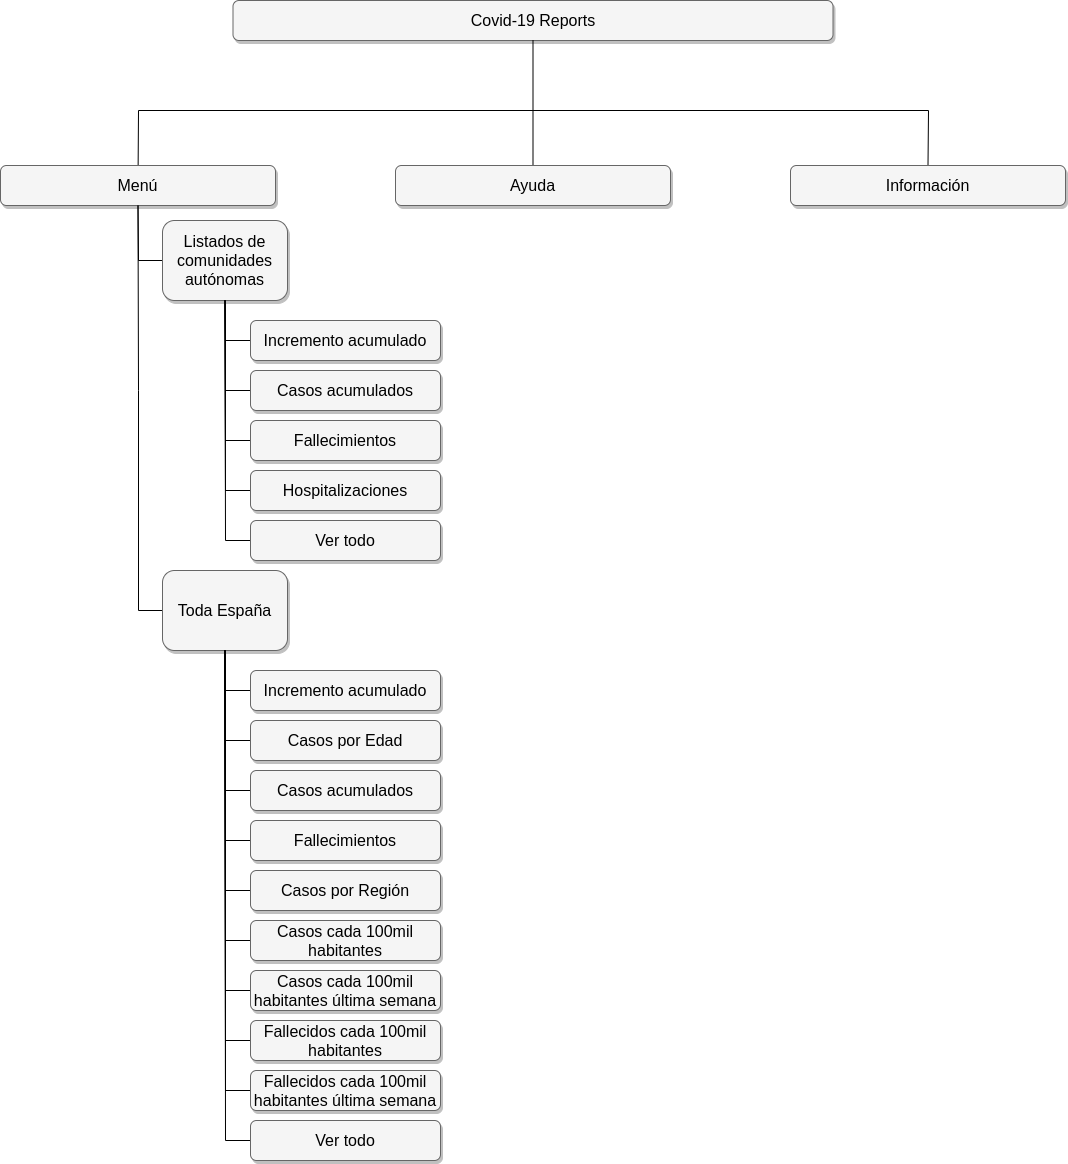
\includegraphics[width=0.9\textwidth]{img/sitemap}
	\caption{Sitemap del Bot.}
	\label{fig:sitemap}
\end{figure}

\subsection{Diseño del wireframe}

El \textbf{wireframe} es un boceto donde se representan visualmente de manera sencilla y estemática la estructura de una web. En este caso . Las Figuras \ref{fig:boceto1} a \ref{fig:boceto12} representan la estructura de \textbf{Covid-19 Reports}.

\begin{figure}[H]
	\centering
	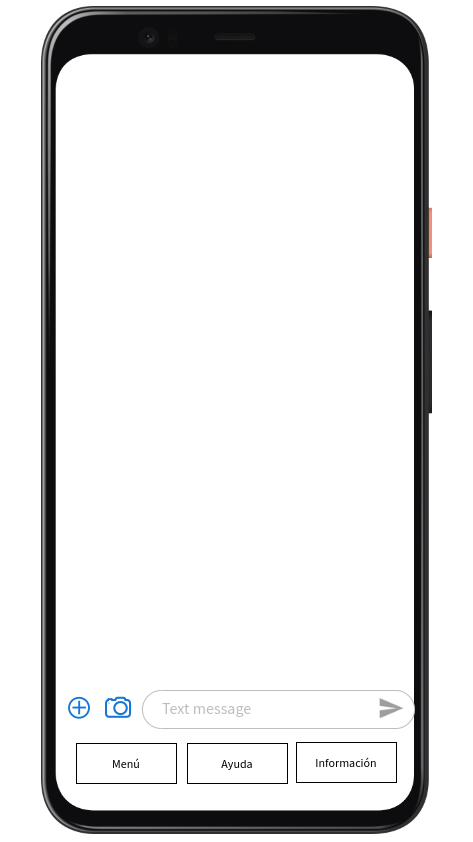
\includegraphics[width=0.75\textwidth]{img/boceto-inicio}
	\caption{Boceto de la pantalla principal.}
	\label{fig:boceto1}
\end{figure}

\begin{figure}[p]
	\centering
	\includegraphics[width=0.75\textwidth]{img/boceto-menú}
	\caption{Boceto Menú principal de selección.}
	\label{fig:boceto2}
\end{figure}

\begin{figure}[p]
	\centering
	\includegraphics[width=0.75\textwidth]{img/boceto-menú-comunidad}
	\caption{Boceto Menú Comunidad Autónoma.}
	\label{fig:boceto3}
\end{figure}

\begin{figure}[p]
	\centering
	\includegraphics[width=1.1\textwidth]{img/boceto-menú-incremento-acumulados}
	\caption{Boceto Menús Incremento y Casos acumulados.}
	\label{fig:boceto4}
\end{figure}

\begin{figure}[p]
	\centering
	\includegraphics[width=1.1\textwidth]{img/boceto-menú-fallecidos-hospitalizados}
	\caption{Boceto Menús Fallecidos y Hospitalizaciones.}
	\label{fig:boceto5}
\end{figure}

\begin{figure}[p]
	\centering
	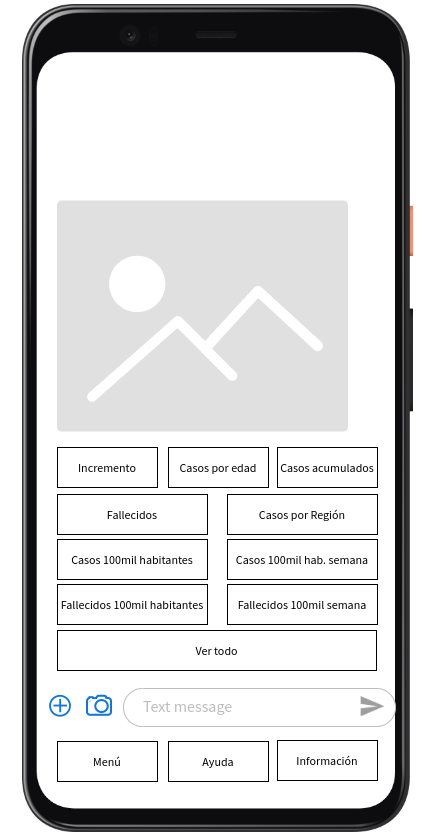
\includegraphics[width=1.1\textwidth]{img/boceto-menú-españa}
	\caption{Boceto Menú España.}
	\label{fig:boceto6}
\end{figure}

\begin{figure}[p]
	\centering
	\includegraphics[width=1.1\textwidth]{img/boceto-menú-es-incremento-edad}
	\caption{Boceto Menús Incremento y Casos por edad en España.}
	\label{fig:boceto7}
\end{figure}

\begin{figure}[p]
	\centering
	\includegraphics[width=1.1\textwidth]{img/boceto-menú-es-acumulados-fallecidos}
	\caption{Boceto Menús Casos acumulados y Fallecidos en España.}
	\label{fig:boceto8}
\end{figure}

\begin{figure}[p]
	\centering
	\includegraphics[width=1.1\textwidth]{img/boceto-menú-es-region-c100}
	\caption{Boceto Menús Casos por Región y Casos cada 100mil habitantes en España.}
	\label{fig:boceto9}
\end{figure}

\begin{figure}[p]
	\centering
	\includegraphics[width=1.1\textwidth]{img/boceto-menú-es-c100s-f100}
	\caption{Boceto Menús Casos cada 100mil hab. semana y Fallecidos cada 100mil habitantes en España.}
	\label{fig:boceto10}
\end{figure}

\begin{figure}[p]
	\centering
	\includegraphics[width=1.1\textwidth]{img/boceto-menú-es-f100s}
	\caption{Boceto Menú Fallecidos cada 100mil hab. semana en España.}
	\label{fig:boceto11}
\end{figure}

\begin{figure}[p]
	\centering
	\includegraphics[width=1.1\textwidth]{img/boceto-menú-ayuda-info}
	\caption{Boceto Menús Ayuda e Información.}
	\label{fig:boceto12}
\end{figure}

Como hemos visto, a lo largo de este capítulo se han mostrados los diferentes puntos del análisis del proyecto, los cuales nos serán útiles a la hora de llevar a cabo del mismo. En el próximo capítulo se muestra como se ha llevado a cabo la implementación del proyecto siguiendo las bases que se han desarrollado.

	% Desarrollo bajo sprints: 
	% 	1. Permitir registros y login de usuarios
	% 	2. Desarrollo del sistema de incidencias
	% 	3. Desarrollo del sistema de denuncias administrativas y accidentes
	% 	4. Desarrollo del sistema de croquis
	%   5. Instalación de la aplicación de manera automática
	\chapter{Implementación}

Como ya se explicó en el Capítulo \ref{ch:planificación} la implementación del proyecto se ha llevado a cabo en una serie de \textbf{Sprints}. Estos se han definido en \textbf{GitHub} a modo de \textit{hitos} y cada uno de ellos contendrá un grupo de \textit{issues} que corresponden a las diferentes \textbf{Historias de Usuario} y \textbf{Tareas} que se han ido incorporando al proyecto a lo largo desarrollo del mismo. \\

\section{Creación del Bot}

La creación de un Bot de \textbf{Telegram} es un proceso muy simple, ya que podemos hacerlos desde la propia aplicación. \textbf{Telegram} tiene su propio Bot implementado que permite crear el resto de estos, este es \textbf{@BotFather}. Al iniciar la comunicación con este Bot lo primero que se nos dará será un listado de las diferentes opciones de las que disponemos para crear, editar, eliminar un Bot entre otras, como puede verse en la Figura \ref{fig:crear-bot-1}.

\begin{figure}[p]
	\centering
	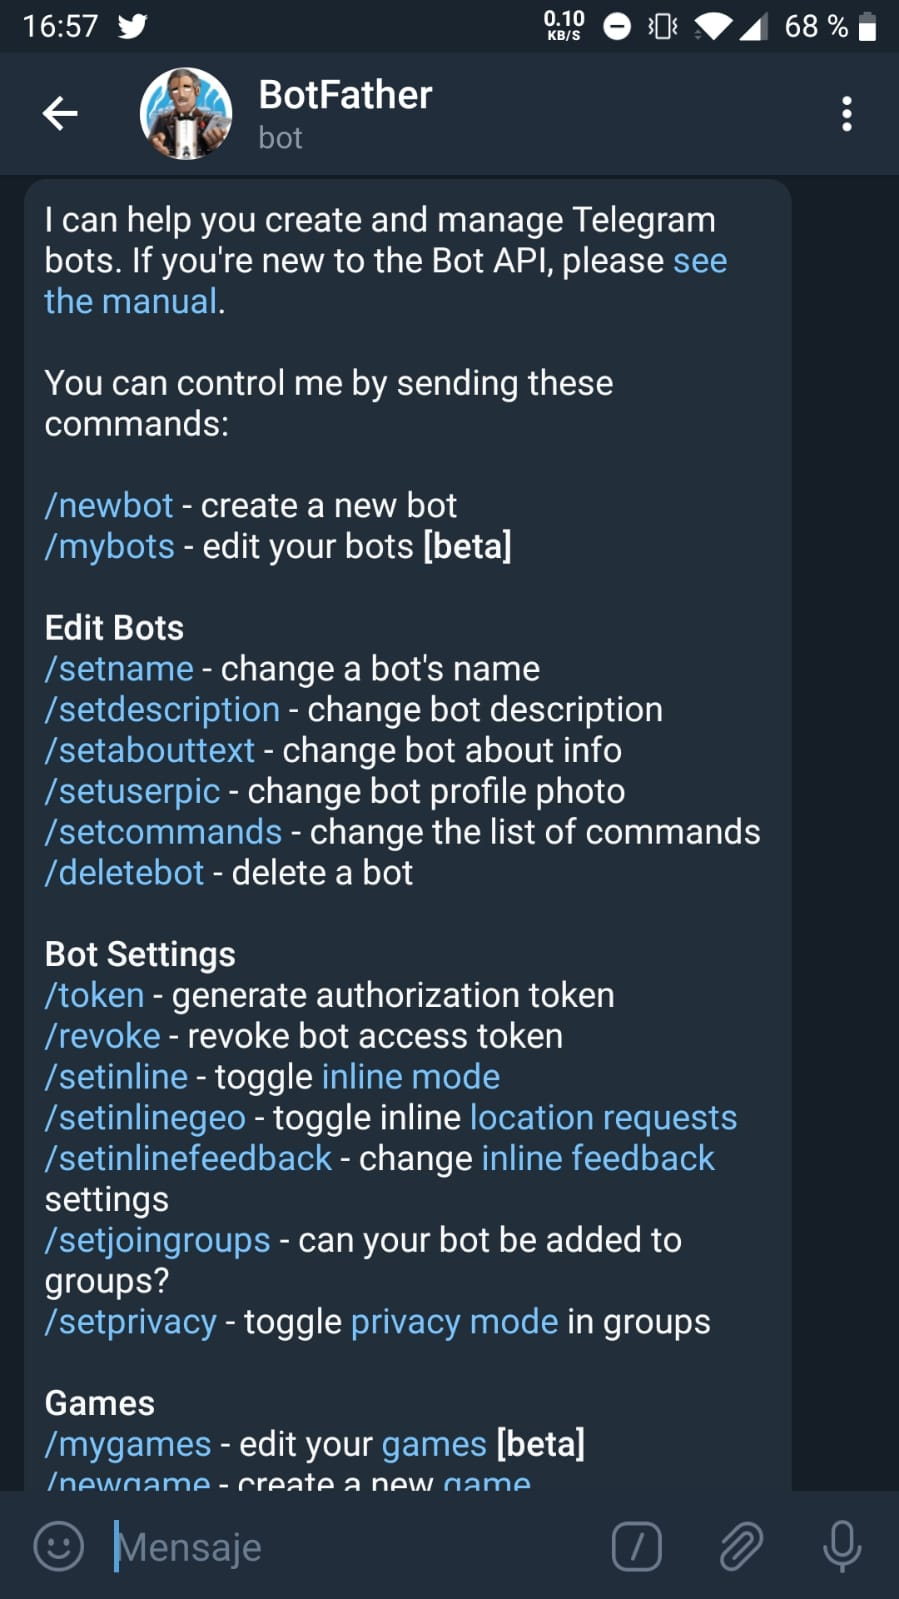
\includegraphics[width=0.8\textwidth]{img/crear-bot-1}
	\caption{Opciones disponibles de @BotFather.}
	\label{fig:crear-bot-1}
\end{figure}

Para crear el Bot tendremos que seleccionar (o escribir) el comando \textbf{/newbot} y el propio \textbf{BotFather} nos pedirá el nombre que queremos darle junto con el nombre de usuario que tendrá en \textbf{Telegram} (terminando este siempre en "bot"). Tras introducirlos, \textbf{BotFather} nos proveerá del TOKEN necesario para poder acceder a la API de \textbf{Telegram} con nuestro Bot, como puede verse en la Figura \ref{fig:crear-bot-2}

\begin{figure}[p]
	\centering
	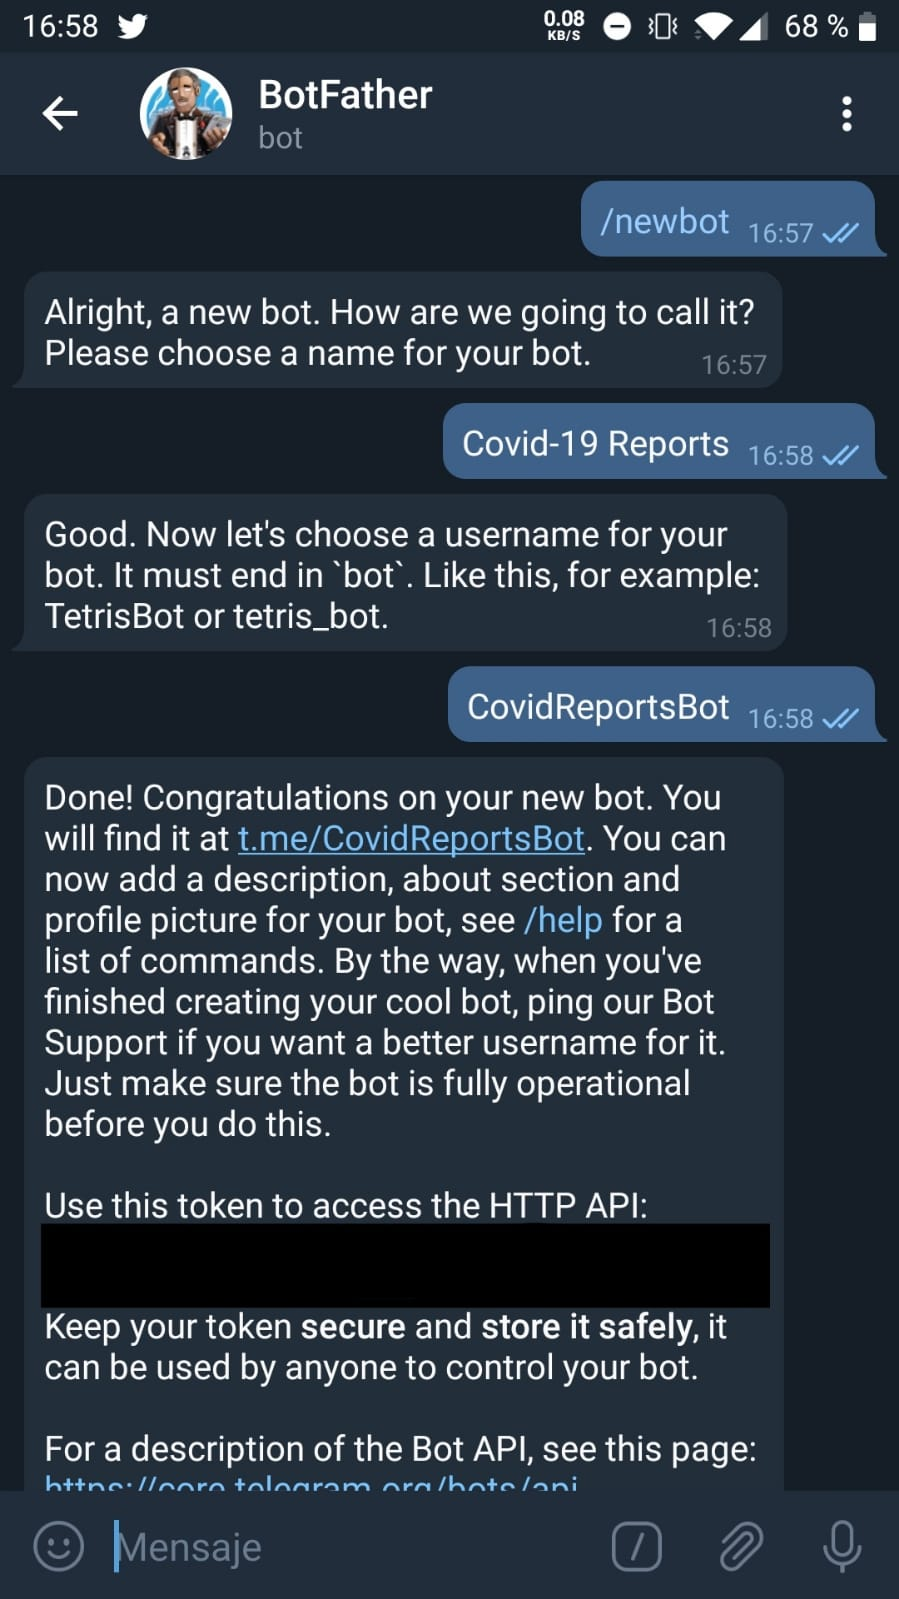
\includegraphics[width=0.8\textwidth]{img/crear-bot-2}
	\caption{Creación del Bot.}
	\label{fig:crear-bot-2}
\end{figure}

Como ya se mencionó en la Sección \ref{sec:recursos}, usaremos la biblioteca \textbf{python-telegram-bot} para implementar el Bot, así como \textbf{Heroku} para llevar a clavo su despliegue. Como base para desarrollar el Bot se tomó el artículo de Artem Rys \cite{crear-bot-heroku} donde se nos explica como crear un Bot haciendo uso de esta biblioteca y como configurar \textbf{Heroku} para su despliegue en la plataforma.

\section{Implementación del Bot}

A lo largo de este apartado se explicarán como se ha llevado a cabo la implementación del Bot mostrando código del mismo.

\subsection{Handlers}

Para poder manejar las diferentes acciones que realizará el Bot se ha hecho uso de una serie de \textbf{handlers} que nos proporciona la propia biblioteca \textbf{python-telegram-bot}. En este caso, entre los diferentes \textbf{handlers} que puede proveernos esta biblioteca a lo largo del proyecto se han utilizado los siguientes:

\begin{itemize}
	\item \textbf{CallbackQueryHandler:} con la siguiente estructura en su llamada \textit{CallbackQueryHandler(callback, pattern), este handler se encargará de ejecutar la función definida en el \textit{callback} cuando se pulse un botón cuyo \textit{pattern} coincide con el del handler.
	\item \textbf{CommandHandler:} con la siguiente estructura en su llamada \textit{CommandHandler(command, callback)}, este handler se encargará de de ejecutar la función definida en el \textit{callback} cuando reciba el \textit{command} (comando)) correcto (los comandos de \textbf{Telegram} son aquellos mensajes que comienzan por \textbf{/}).
	\item \textbf{MessageHandler:} con la siguiente estructura en su llamada \textit{MessageHandler(filters, callback)}, este handler se encargará de de ejecutar la función definida en el \textit{callback} cuando reciba reciba un mensaje que cumpla con las condiciones definidas en su \textit{filters} (filtros)}.
\end{itemize}

\subsection{Funciones de respuesta}

Como hemos dicho con anterioridad, este Bot será de tipo conversacional. Esto conlleva que el Bot tendrá que responder a las solicitudes que el usuario le realice. Para ello se han definido una serie de funciones que, haciendo uso de los \textbf{handlers} definidos en el apartado anterior compondrán nuestro Bot, permitiendo responder al usuario.

Estas funciones estarán caracterizadas por estar definidas todas con dos parámetros (\textbf{update} y \textbf{context}) los cuales contienen información del mensaje enviado (nombre y apellidos del usuario, alias, identificador del chat). Podemos verlo en el Listing \ref{lst:def-funcion}

\lstset{
	backgroundcolor=\color{white},
	basicstyle=\footnotesize,
	breakatwhitespace=false,         
	breaklines=true,
	captionpos=b,
	commentstyle=\color{green},
	extendedchars=true,              
	frame=single,
	keepspaces=true,
	keywordstyle=\color{blue},
	language=Python,
	numbers=left,
	numbersep=5pt,
	numberstyle=\small\color{black},
	showstringspaces=false,
	rulecolor=\color{black},
	stringstyle=\color{blue},
	tabsize=2,
	texcl=true
}

\begin{lstlisting}[language=Python, caption={Definición de un función usada por los handler.}, label={lst:def-funcion}]
def nombre_funcion ( update , context ) :
\end{lstlisting}

Para facilitar el entendimiento, mostraremos los diferentes modelos de funciones que se han utilizado para implementar el Bot, evitando así exponer todo el código del mismo ya que la estructura de las funciones es la misma dependiendo del tipo. Dentro de los diferentes tipos de funciones implementada, las dividiremos según el tipo de respuestas que estas nos ofrecen.

\subsubsection{Función para iniciar el Bot}

La primera función que definirá el Bot será su funcionó de inicio, la cual permitirá poder empezar a utilizar el Bot y creará los botones de los menús en el teclado del usuario. Desglosaremos el código del Listing \ref{lst:def-funcion-inicio}:

\begin{itemize}
	\item \textbf{Lineas 1 y 2:} Recogen en dos variables los valores del nombre del usuario y el identificador del chat desde los parámetros.
	\item \textbf{Lineas 4 a 7:} Comprueba que el usurario tiene un usuario de \textbf{Telegram} y si no lo tiene le informa de como hacerlo.
	\item \textbf{Lineas 11 a 13:} Se crea una lista con los botones del teclado que se quieren mostrar al usuario. A diferencia de los botones que se muestran en el chat, estos carecen de un parámetro \textbf{callback\_data}.
	\item \textbf{Lineas 15 a 17:} Se crea el objeto que contendrá los botones y se le especifica que quiere que se adapte al tamaño del teclado (\textbf{resize\_keyboard}), así como que quiere que siempre se mantenga visible (\textbf{one\_time\_keyboard}).
	\item \textbf{Lineas 19 a 22:} Se usará la función \textbf{reply\_text} sobre el mensaje que nos da el Bot para añadirle el texto que queremos que este devuelva, asi como un parámetro adicional (\textbf{reply\_markup}) donde se encuentra el listado de botones del menú del teclado.
\end{itemize}

\begin{lstlisting}[language=Python, caption={Función de inicio del Bot.}, label={lst:def-funcion-inicio}]
chat_id = update.effective_user["id"]
username = update.message.chat.username

if username is None:
	logger.info("User {} started bot".format('None:' + str(chat_id)))
	update.message.reply_text("Bienvenido a Covid-19 Report! Parece que no tienes usuario de Telegram."
							  " Ve a ajustes, ponte un nombre de usuario y podremos empezar.")
else:
	logger.info("User {} started bot".format(username + ':' + str(chat_id)))

	main_menu_keyboard = [[KeyboardButton("Menu"),
						   KeyboardButton("Ayuda"),
						   KeyboardButton("Informacion")]]

	reply_kb_markup = ReplyKeyboardMarkup(main_menu_keyboard,
										  resize_keyboard=True,
										  one_time_keyboard=False)

update.message.reply_text(text="Bienvenido a Covid-19 Report! {}\n"
							   "Gracias a este bot podras conocer el estado de la situacion actual provocada "
							   "por el Covid-19.".format(username),
						  reply_markup=reply_kb_markup)
\end{lstlisting}

\subsubsection{Función responde con texto}

En este apartado analizaremos como que implementa una función para cuando el Bot solo devuelva texto. Desglosaremos el código del Listing \ref{lst:def-funcion-texto}:

\begin{itemize}
	\item \textbf{Lineas 1:} Se usará la función \textbf{reply\_text} para añadirle el texto que se quiere que el Bot devuelva cuando el \textbf{handler} llame a la función.
\end{itemize}

\begin{lstlisting}[language=Python, caption={Función que devuelve texto en el chat.}, label={lst:def-funcion-texto}]
update.message.reply_text("Usa /start para iniciar el bot")
\end{lstlisting}

\subsubsection{Función responde con texto y botones}

En este apartado analizaremos como que implementa una función para cuando el Bot devuelva texto y botones. Desglosaremos el código del Listing \ref{lst:def-funcion-texto-botones}:

\begin{itemize}
	\item \textbf{Lineas 1 a 6:} Se creará una lista con los botones que el Bot mostrará al usuario. Estos contendrán un parámetro \textbf{callback\_data} donde se definirá el nombre del callback para que al pulsar el botón el \textbf{handler CallbackQueryHandler} ejecute la función asociada a este callback.
	\item \textbf{Lineas 8 a 11:} Se usará la función \textbf{reply\_text} para añadirle el texto que se quiere que el Bot devuelva cuando el \textbf{handler} llame a la función, asi como un parámetro adicional (\textbf{reply\_markup}) donde se encuentra el listado de botones que mostrará el Bot en el chat.
\end{itemize}

\begin{lstlisting}[language=Python, caption={Función que devuelve texto y botones en el chat.}, label={lst:def-funcion-texto-botones}]
keyboard = [
	[InlineKeyboardButton("Andalucia", callback_data='andalucia_info'),
	InlineKeyboardButton("Aragon", callback_data='aragon_info'),
	InlineKeyboardButton("Asturias", callback_data='asturias_info')],
	]
reply_markup = InlineKeyboardMarkup(keyboard)

message.reply_text(
	text="{} elige la comunidad de la que quieres consultar datos.".format(username),
	reply_markup=reply_markup
)
\end{lstlisting}

\subsubsection{Función responde con imagen}

En este apartado analizaremos como que implementa una función para cuando el Bot solo devuelva texto. Desglosaremos el código del Listing \ref{lst:def-funcion-imagen}:

\begin{itemize}
	\item \textbf{Lineas 1:} Se usará la función \textbf{reply\_text} hacer que el Bot envía la imagen al chat cuando el \textbf{handler} llame a la función que contiene el código.
	\item \textbf{Lineas 2:} Se usará la función \textbf{open} para abrir la imagen que se encuentra en la \textbf{ruta}, indicando el parámetro \textbf{rb} que se abrirá con representación binaria
\end{itemize}

\begin{lstlisting}[language=Python, caption={Función que devuelve una imagen en el chat.}, label={lst:def-funcion-imagen}]
message.reply_photo(
	photo=open('ruta', 'rb')
)
\end{lstlisting}

\subsection{Fallbacks}

Al tratarse de un Bot conversacional, una de las cosas principales que se ha de tener en cuenta en el momento de su implementación es que este no puede dar información que no corresponda con el contexto en el que se encuentra. Un ejemplo en \textbf{Covid-19 Reports} sería estando en el contexto de consulta de los datos una provincia, preguntarle por la información de los casos de España.

Ahora pasaremos a mostrar como funcionan los \textbf{fallbacks}. En primer lugar, se han definido una serie de \textbf{contextos} sobre los que el Bot puede actuar. Un ejemplo de estos seria el contexto \textbf{INICIO}, donde definiremos los diferentes \textbf{handler} con las respuestas posibles que el Bot podría darnos en este contexto como se muestra en el Listing \ref{lst:contexto}

\begin{lstlisting}[language=Python, caption={Lista de handlers asociado al conexto INICIO.}, label={lst:contexto}]
INICIO: [
	MessageHandler(Filters.regex('Menu'), show_inicio),
	MessageHandler(Filters.regex('Ayuda'), help_handler),
	MessageHandler(Filters.regex('Informacion'), show_info),
	MessageHandler(Filters.text & (~Filters.command), any_message),
	CallbackQueryHandler(show_andalucia_info, pattern='andalucia_info'),
	CallbackQueryHandler(show_aragon_info, pattern='aragon_info'),
	CallbackQueryHandler(show_asturias_info, pattern='asturias_info'),
	CallbackQueryHandler(show_cvalenciana_info, pattern='cvalenciana_info'),
	CallbackQueryHandler(show_canarias_info, pattern='canarias_info'),
	CallbackQueryHandler(show_cantabria_info, pattern='cantabria_info'),
	CallbackQueryHandler(show_castillalamancha_info, pattern='castillalamancha_info'),
	CallbackQueryHandler(show_castillayleon_info, pattern='castillayleon_info'),
	CallbackQueryHandler(show_cataluna_info, pattern='cataluna_info'),
	CallbackQueryHandler(show_ceuta_info, pattern='ceuta_info'),
	CallbackQueryHandler(show_extremadura_info, pattern='extremadura_info'),
	CallbackQueryHandler(show_galicia_info, pattern='galicia_info'),
	CallbackQueryHandler(show_baleares_info, pattern='baleares_info'),
	CallbackQueryHandler(show_larioja_info, pattern='larioja_info'),
	CallbackQueryHandler(show_madrid_info, pattern='madrid_info'),
	CallbackQueryHandler(show_melilla_info, pattern='melilla_info'),
	CallbackQueryHandler(show_murcia_info, pattern='murcia_info'),
	CallbackQueryHandler(show_navarra_info, pattern='navarra_info'),
	CallbackQueryHandler(show_paisvasco_info, pattern='paisvasco_info'),
	CallbackQueryHandler(show_espana_info, pattern='espana_info'),
],
\end{lstlisting}

Como se puede ver, en este contexto el Bot presenta una diversidad de opciones asociadas tanto a botones como con texto que se puede introducir. Pero, ¿que pasa si se produce un acción en otro contexto? Para ello existen los \textbf{fallbacks}. Éstos estarán representados en una lista donde se implementarán los \textbf{handlers} que no se encuentran en el contexto correcto. Por ello, como podremos ver en el Listing \ref{lst:fallback}, se han definido los mismos \textbf{handlers} implementados en el Listing \ref{lst:contexto}. Esto es porque estos mismos handlers pueden no corresponder a cualquier otro contexto, por lo que el \textbf{fallback} asociado al \textbf{pattern} se encargará de llamar a otra función diferente a la original de manera que se realice una acción diferente. Para \textbf{Covid-19 Reports}, esa opción será la de mostrar un mensaje comunicando que no se encuentra en el contexto de la petición.

\begin{lstlisting}[language=Python, caption={Fallbacks.}, label={lst:fallback}]
INICIO: [
	CommandHandler('start', start_handler),
	CommandHandler('help', help_handler),
	CommandHandler('info', show_info),
	CallbackQueryHandler(usuario_pulsa_boton_anterior,
	pattern='start_menu'),
	CallbackQueryHandler(usuario_pulsa_boton_anterior, pattern='andalucia_info'),
	CallbackQueryHandler(usuario_pulsa_boton_anterior, pattern='aragon_info'),
	CallbackQueryHandler(usuario_pulsa_boton_anterior, pattern='asturias_info'),
	CallbackQueryHandler(usuario_pulsa_boton_anterior, pattern='cvalenciana_info'),
	CallbackQueryHandler(usuario_pulsa_boton_anterior, pattern='canarias_info'),
	CallbackQueryHandler(usuario_pulsa_boton_anterior, pattern='cantabria_info'),
	CallbackQueryHandler(usuario_pulsa_boton_anterior, pattern='castillalamancha_info'),
	CallbackQueryHandler(usuario_pulsa_boton_anterior, pattern='castillayleon_info'),
	CallbackQueryHandler(usuario_pulsa_boton_anterior, pattern='cataluna_info'),
	CallbackQueryHandler(usuario_pulsa_boton_anterior, pattern='ceuta_info'),
	CallbackQueryHandler(usuario_pulsa_boton_anterior, pattern='extremadura_info'),
	CallbackQueryHandler(usuario_pulsa_boton_anterior, pattern='galicia_info'),
	CallbackQueryHandler(usuario_pulsa_boton_anterior, pattern='baleares_info'),
	CallbackQueryHandler(usuario_pulsa_boton_anterior, pattern='larioja_info'),
	CallbackQueryHandler(usuario_pulsa_boton_anterior, pattern='madrid_info'),
	CallbackQueryHandler(usuario_pulsa_boton_anterior, pattern='melilla_info'),
	CallbackQueryHandler(usuario_pulsa_boton_anterior, pattern='murcia_info'),
	CallbackQueryHandler(usuario_pulsa_boton_anterior, pattern='navarra_info'),
	CallbackQueryHandler(usuario_pulsa_boton_anterior, pattern='paisvasco_info'),
	CallbackQueryHandler(usuario_pulsa_boton_anterior, pattern='espana_info'),
],
\end{lstlisting}

Como puede verse, también se han usado algunos \textbf{CommandHandler}, dado que queremos permitir que en cualquier contexto estos puedan llamar a sus respectivas funciones.

\subsection{Funciones análisis de datos}

Para poder llevar a cabo la implementación del análisis de datos, en primer lugar, debemos saber como están estos datos estructurados. Los datos que se van a utilizar para implementar el Bot los conseguiremos desde el \textbf{GitHub de Datadista} \cite{github-datadista}. Al tratarse de archivos tipo \textit{.csv} se optó por hacer uso de la librería \textbf{pandas} como se dijo en la Sección \ref{sec:recursos}.

Para poder cargar la información de estos archivos se usará la función de \textbf{pandas} \textbf{read\_csv}, pudiendo ver un ejemplo en el Listing \ref{lst:read-csv}. De los parámetros que se utilizan en esta función, \textbf{usecols} es el único que no se usa en todos los casos, dado que éste sirve para indicar, mediante una lista, las columnas que se querrán cargar en el \textbf{dataframe}. Los otros dos parámetros nos indicarán, en primer lugar conde se puede encontrar el archivo, ya sea en una ruta definida en algún directorio como una url que contenga los datos, y el parámetro \textbf{sep} indicará cual es el caracter separador a tener en cuenta.

\begin{lstlisting}[language=Python, caption={Función read\_csv.}, label={lst:read-csv}]
df = pd.read_csv('ruta/url', sep=',', usecols=list_columns)
\end{lstlisting}

Una vez cargados los datos en sus correspondientes \textbf{dataframes} se procede a trabajar con ellos para obtener los datos que queremos que el Bot devuelva al usuario.

Para un mayor claridad, explicaremos la estructura de los diferentes \textbf{dataframes} y lo que representa cada uno de sus valores.

\subsubsection{Dataframe casos por Comunidad Autónoma}

Este \textbf{dataframe} contendrá la información del nº de casos que se han producido en cada Comunidad Autónoma en una fecha concreta. Éste tendrá la siguiente estructura:

\begin{center}
	\textit{(fecha, ccaa, num\_casos)}
\end{center}

\begin{itemize}
	\item \textbf{fecha:} clave principal, fecha en formato YYYY-mm-dd.
	\item \textbf{ccaa:} nombre de la Comunidad Autónoma.
	\item \textbf{num\_casos:} nº de casos detectados en la Comunidad Autónoma en la fecha.
\end{itemize}

\subsubsection{Dataframe fallecidos por Comunidad Autónoma}

Este \textbf{dataframe} contendrá la información del nº de fallecimientos que se han producido en cada Comunidad Autónoma en una fecha concreta. Éste tendrá la siguiente estructura:

\begin{center}
	\textit{(Fecha, CCAA, Fallecidos)}
\end{center}

\begin{itemize}
	\item \textbf{Fecha:} clave principal, fecha en formato YYYY-mm-dd.
	\item \textbf{CCAA:} nombre de la Comunidad Autónoma.
	\item \textbf{Fallecidos:} nº de fallecidos confirmados en la Comunidad Autónoma en la fecha.
\end{itemize}

\subsubsection{Dataframe datos hospitalización por Comunidad Autónoma}

Este \textbf{dataframe} contendrá la información de los datos hospitalarios que se han producido en cada Comunidad Autónoma y en España en una fecha concreta. Éste tendrá la siguiente estructura:

\begin{center}
	\textit{(Fecha, CCAA, Total Pacientes COVID ingresados, \% Camas Ocupadas COVID, Total pacientes COVID en UCI, \% Camas Ocupadas UCI COVID, Ingresos COVID últimas 24 h, Altas COVID últimas 24 h)}
\end{center}

\begin{itemize}
	\item \textbf{Fecha:} clave principal, fecha en formato YYYY-mm-dd.
	\item \textbf{CCAA:} nombre de la Comunidad Autónoma (o España).
	\item \textbf{Total Pacientes COVID ingresados:} nº de pacientes Covid que se encuentran hospitalizados en la fecha.
	\item \textbf{\% Camas Ocupadas COVID:} \% de las camas disponibles en hospitales ocupada por pacientes Covid en la fecha.
	\item \textbf{Total pacientes COVID en UCI:} nº de pacientes Covid que se encuentran hospitalizados en UCI en la fecha.
	\item \textbf{\% Camas Ocupadas UCI COVID:} \% de las camas UCI disponibles en hospitales ocupada por pacientes Covid en la fecha.
	\item \textbf{Ingresos COVID últimas 24 h:} nº de pacientes ingresados en las últimas 24 horas en la fecha.
	\item \textbf{Altas COVID últimas 24 h:} nº de pacientes dados de alta en las últimas 24 horas en la fecha.
\end{itemize}

\subsubsection{Dataframe casos y fallecimiento por rango de edad}

Este \textbf{dataframe} contendrá la información del nº de casos y fallecidos que se han producido en el país por rango de edad y sexo en una fecha concreta. Éste tendrá la siguiente estructura:

\begin{center}
	\textit{(fecha, rango\_edad, sexo, casos\_confirmados, hospitalizados, ingresos\_uci, fallecidos)}
\end{center}

\begin{itemize}
	\item \textbf{fecha:} clave principal, fecha en formato YYYY-mm-dd.
	\item \textbf{rango\_edad:} rango de edad donde se han producido los casos, divididos en intervalos de 10 años, desde \textit{0-9} hasta \textit{80 y +}. También existe un \textit{Total} de los datos.
	\item \textbf{sexo:} indicará el sexo de la población, dividiéndose en \textit{hombres}, \textit{mujeres} y \textit{ambos}.
	\item \textbf{casos\_confirmados:} nº de casos detectados por edad y rango en la fecha.
	\item \textbf{hospitalizados:} nº de pacientes Covid hospitalizados por edad y rango en la fecha.
	\item \textbf{ingresos\_uci:} nº de pacientes Covid hospitalizados en UCI por edad y rango en la fecha.
	\item \textbf{fallecidos:} nº de fallecidos confirmados por edad y rango en la fecha.
\end{itemize}

\subsubsection{Dataframe nº de habitantes por Comunidad Autónoma}

Este \textbf{dataframe} contendrá la información del nº de habitantes de cada Comunidad Autónoma. Éste tendrá la siguiente estructura:

\begin{center}
	\textit{(ccaa, habitantes)}
\end{center}

\begin{itemize}
	\item \textbf{ccaa:} clave principal, nombre de cada Comunidad Autónoma de España.
	\item \textbf{habitantes:} nº total de habitantes de cada Comunidad Autónoma.
\end{itemize}

Para evitar repetir el código, se mostrará las funciones que se usan sobre estos \textbf{dataframes} a lo largo del proyecto presentándolos en los Listing \ref{lst:funcion-1} a \ref{lst:funcion-2}.

En el Listing \ref{lst:funcion-1} se muestra el uso de dos funciones, \textbf{groupby} y \textbf{sum}, las cuales en el ejemplo, se usan para poder devolver la sumatoria de los casos agrupados por Comunidades, seleccionando por último la Comunidad de la que se quiere conocer la sumatoria de sus casos.

\begin{itemize}
	\item \textbf{Función groupby:} Esta será la encargada de agrupar los datos según la columna elegida, la cual no identifica a la clave del dataframe, en este caso la columna \textit{ccaa}. 
	\item \textbf{Función sum:} Ésta será la encargada de realizar la sumatoria de los valores seleccionados. Es este ejemplo, tras agrupar los datos por Comunidades, se realizará la sumatoria del nº de casos de las mismas.
\end{itemize}

\begin{lstlisting}[language=Python, caption={Funciones groupby y sum.}, label={lst:funcion-1}]
df_ccaa_casos.groupby(['ccaa'])['num_casos'].sum()[current_autonomy]
\end{lstlisting}

En el Listing \ref{lst:funcion-2} se muestra el uso de la función \textbf{loc}. Ésta se usa a lo largo del proyecto para crear nuevos dataframes que cumplan una serie de condiciones simultaneas, por ejemplo, seleccionar los datos de una Comunidad concreta en una fecha deseada.

\begin{itemize}
	\item \textbf{Función loc:} Esta será la encargada de, por medio de las condiciones definidad en si interior, crear un nuevo dataframe que cumpla las mismas.
	\item \textbf{Values:} Values se usará para obtener el valor de una columna, es este caso, el primer valor de la comuna \textit{col}.
\end{itemize}

\begin{lstlisting}[language=Python, caption={Función loc.}, label={lst:funcion-2}]
df_loc = df.loc[(condicion_1) & (condicion_2)]

df_loc['col'].values[0]
\end{lstlisting}

Por medio de estas funciones se hará una selección de los datos que el Bot ha demostrar al usuario, pudiendo combinarlas entre ellas para obtener diferentes datos.

\subsection{Funciones de creación de gráficas}

Para permitir que el Bot pueda crear diferentes imágenes que muestren gráficos y las muestre junto a los datos que se obtienen en el punto anterior se ha hecho uso de la biblioteca \textbf{matplotlib}. Esta nos permitirá crear gráficos haciendo uso de los datos de los \textbf{dataframes}.

Existen diferentes tipos de gráficos que se pueden usar. Para este proyecto dependiendo del los tipos de datos se han elegido diferentes modelos de gráficos: barras, barras laterales, tramas.

\subsubsection{Gráficos de barras y tramas}

Para los gráficos de barras y tramas se ha seguido la estructura que de muestra en el Listing \ref{lst:barras}. 

\begin{itemize}
	\item \textbf{Lineas 1 y 2:} Se creará creará un nuevo \textbf{dataframe} con los datos de los que se desea mostrar y por medio de la función \textbf{set\_index} se asignará la columna del \textbf{dataframe} como el index del mismo.
	\item \textbf{Lineas 4:} Se creará el tamaño de la imagen y se crearán las variables \textbf{fig} y \textbf{ax} que se usarán mas adelante.
	\item \textbf{Lineas 5:} Se creará una variable que contendrá un objeto \textit{Index} que será el que contenga los indices de la gráfica.
	\item \textbf{Lineas 7:} Se creará la gráfica de barras, donde los parámetros introducisos serán el Index creado antes, el listado de valores correspondientes a cada index, así como la opacidad de la barra (alpha) y el grosor de éstas (width).
	\item \textbf{Lineas 8:} Se creará la gráfica de tramas, donde los parámetros introducisos serán el Index creado antes, el listado de valores correspondientes a cada index, así como el color de la misma.
	\item \textbf{Lineas 10:} Se indicarán los valores que se representarán en el axis de la gráfica.
	\item \textbf{Lineas 11:} Se indicarán los valores de inicio y final que se representarán en el axis de la gráfica.
	\item \textbf{Lineas 12:} Se formateará como se muestras los diferentes valores de axis.
	\item \textbf{Lineas 14 y 15:} Se le da nombre a la gráfica así como a su eje y.
	\item \textbf{Lineas 16 y 17:} Crea el archivo con la gráfica en el directorio seleccionado y posteriormente cerraremos la figura para evitar problemas al crear otras gráficas.
\end{itemize}

\begin{lstlisting}[language=Python, caption={Generár gráficos de barras y tramas.}, label={lst:barras}]
df_casos_fecha = df_ccaa_casos.groupby('fecha')['num_casos'].sum().reset_index()
df_casos_fecha.set_index("fecha", inplace=True)

fig, ax = plt.subplots(figsize=(12, 6))
x = df_casos_fecha.index.get_level_values('fecha')

plt.bar(x, df_casos_fecha['num_casos'], alpha=0.5, width=0.5)
plt.plot(x, df_casos_fecha['num_casos'], color='red')

ax.set_xticks(inicio_mes)
ax.set_xlim('2020-03-01', x[-1])
ax.figure.autofmt_xdate()

plt.title('Incremento de casos en Espana', fontsize=26)
ax.set_ylabel('N Casos', fontsize=15)
plt.savefig('./img_graficas/incremento_espana.png')
plt.close()
\end{lstlisting}

\subsubsection{Gráficos de barras laterales}

Para los gráficos de barras y tramas se ha seguido la estructura que de muestra en el Listing \ref{lst:barras-laterales}. 

\begin{itemize}
	\item \textbf{Lineas 1 y 2:} Se creará creará un nuevo \textbf{dataframe} con los datos de los que se desea mostrar y por medio de la función \textbf{set\_index} se asignará la columna del \textbf{dataframe} como el index del mismo.
	\item \textbf{Lineas 4:} Se creará el tamaño de la imagen y se crearán las variables \textbf{fig} y \textbf{ax} que se usarán mas adelante.
	\item \textbf{Lineas 5:} Se creará una variable que contendrá un objeto \textit{Index} que será el que contenga los indices de la gráfica.
	\item \textbf{Lineas 7:} Se creará la gráfica de barra laterales, donde los parámetros introducidos serán el Index creado antes, el listado de valores correspondientes a cada index, así como la opacidad de la barra (alpha) y el grosor de éstas (width).
	\item \textbf{Lineas 9:} Se formateará como se muestras los diferentes valores de axis.
	\item \textbf{Lineas 11 y 12:} Se le da nombre a la gráfica y se invertirá si eje y.
	\item \textbf{Lineas 14 y 15:} Se le añadirá al final de cada barra el valor que representa la misma.
	\item \textbf{Lineas 17 y 18:} Crea el archivo con la gráfica en el directorio seleccionado y posteriormente cerraremos la figura para evitar problemas al crear otras gráficas.
\end{itemize}

\begin{lstlisting}[language=Python, caption={Generár gráficos de barras laterales.}, label={lst:barras-laterales}]
df_casos_fecha = df_ccaa_casos.groupby('fecha')['num_casos'].sum().reset_index()
df_casos_fecha.set_index("fecha", inplace=True)

fig, ax = plt.subplots(figsize=(12, 6))
x = df_casos_fecha.index.get_level_values('fecha')

plt.barh(x, df['n_casos'], alpha=0.5, height=0.8)

ax.figure.autofmt_xdate()

plt.title('Incremento de casos en Espana', fontsize=26)
plt.gca().invert_yaxis()

for index, value in enumerate(df['n_casos']):
plt.text(value, index, str(value))

plt.savefig('./img_graficas/incremento_espana.png')
plt.close()
\end{lstlisting}



	% Desarrollo bajo sprints: 
	% 	1. Permitir registros y login de usuarios
	% 	2. Desarrollo del sistema de incidencias
	% 	3. Desarrollo del sistema de denuncias administrativas y accidentes
	% 	4. Desarrollo del sistema de croquis
	%   5. Instalación de la aplicación de manera automática
	\chapter{Test y Despliegue}

\section{Desarrollo basado en test}

El desarrollo de test es una de las actividades más importantes y necesarias a la hora de desarrollar un proyecto. Estos se utilizan para poder asegurar la calidad del producto. Al aplicar una metodología como Scrum, se han pretendido que los ciclos de trabajo no sean largos, donde se tengan que arreglar un gran nº de errores a la vez que se añaden nuevas características al producto. Por ello, para minimizar el trabajo lo máximo posible y evitar fallos que pueden llegar a no solucionarse de manera facil.

El desarrollo de test en la teoria ha de preceder al desarrollo del propio código. Los tests se crean partiendo del punto de vista donde ya se conoce las funcionalidades que se van a implementar, como queremos que estas respondan y como medida para estas no fallen al implementarse.

Por esto, para poder afirma que se ha desarrollado un producto funcional, primero este ha de haber pasado una serie de pruebas, las cuales estarán automatizadas por medio de los test. Para el desarrollo de este proyecto se ha hecho uso de dos de estos tipos, ya que ambos son importantes: \textbf{test unitarios} y \textbf{test integrados}. Cada uno de estos test se encargará de realizar pruebas en un aspecto del proyecto.

\subsection{Test unitarios}

Definiremos como \textbf{test unitarios} a aquellos que realizarán pruebas mediante las llamadas de funciones con diferentes valores. Un aspecto a tener en cuenta a la hora de desarrollar pruebas unitarias es que estas siempre han de cubrir todo el código desarrollado, o lo que es lo mismo, tener un \textbf{coverage} del 100\%. Esto se debe a que si dejamos algún punto del código sin testear, este puede darnos algún problema en algún momento y no saberlo porque no se está probando.

Para desarrollar los \textbf{test unitario} de este proyecto se ha utilizado la biblioteca \textbf{pytest}, la cual nos aporta la capacidad de parametrizar el código, de manera que con un mismo test podamos comprobar diferentes casos. Un ejemplo de esto es el test que se muestra en el Listing \ref{lst:unit-test}, donde vemos como se han parametrizado los parámetros del test para comprobar su funcionamiento.

\begin{lstlisting}[language=Python, caption={Ejemplo test unitario parametrizado.}, label={lst:unit-test}]
@pytest.mark.parametrize("fecha,expected", [("2020-12-12", '12-12-2020'), ("0001-07-16", '16-07-1'), ("2098-05-07", '07-05-2098')])
def test_format_date(fecha, expected):
	assert format_date(fecha) == expected
\end{lstlisting}

Como se puede ver, el test recibe los parámetros \textit{fecha} y \textit{expected}, los cuales corresponderán a los valores que se pasarán como parámetro de la función que se va a probar y al resultado que debería devolver la misma.

\subsection{Test integrados}

Definiremos como \textbf{test integrados} a aquellos que realizan pruebas sobre el conjunto del producto una vez este ha pasado satisfactoriamente los test unitarios. Los test integrados serán los encargados de comprobar el funcionamiento completo del proyecto, en nuestro caso, simulando acciones que podría llevar a cabo un usuario.

Para desarrollar los test integrados de este proyecto se ha hecho uso de la biblioteca \textbf{pyrogram}, la cual es una de las que se nos recomienda a la hora de seleccionar \textbf{python-telegram-bot}. Cuenta con una serie de ejemplos en su \textbf{GitHub} los cuales nos permiten probar las diferentes combinaciones en las que se puede realizar esto.

En primer lugar explicaremos el archivo \textit{conftest}, el cual podemos ver en el Listing \ref{lst:conftest} y será el encargado de implementar las funcionalidades principales que luego serán utilizadas para simular un usuario a la hora de realizar los test. 

\begin{itemize}
	\item \textbf{Lineas 1 a 4:} Se habilita el logging y se le asignan los valores que se quieren tener.
	\item \textbf{Lineas 7 a 11:} Se define la función \textit{event\_loop}, la cual crea una instancia del event loop por defecto para la sesión.
	\item \textbf{Lineas 14 a 23:} Se define la función \textit{client}, la cual creará un nuevo cliente para probar el Bot.
	\item \textbf{Lineas 26 a 37:} Se define la función \textit{controller}, la cual se encargará de enviarles las peticiones del cliente al Bot.
\end{itemize}

\begin{lstlisting}[language=Python, caption={Contenido del archivo conftest.}, label={lst:conftest}]
logger = logging.getLogger("test")
logger.setLevel(logging.DEBUG)
logging.basicConfig(level=logging.DEBUG)
logging.getLogger("pyrogram").setLevel(logging.WARNING)


@pytest.yield_fixture(scope="session", autouse=True)
def event_loop(request):
	loop = asyncio.get_event_loop_policy().new_event_loop()
	yield loop
	loop.close()


@pytest.fixture(scope="session")
async def client() -> Client:
	client = Client(
	config("SESSION_STRING", default=None) or "test_covid_reports",
	workdir=test_dir,
	config_file=str(test_dir / "config.ini")
	)
	await client.start()
	yield client
	await client.stop()


@pytest.fixture(scope="module")
async def controller(client):
	c = BotController(
	client=client,
	peer="@CovidReportsBot",
	max_wait=10.0,
	wait_consecutive=0.8, (optional)
	)
	
	await c.clear_chat()
	await c.initialize(start_client=False)
	yield c
\end{lstlisting}

Una ver vista la estructura del archivo \textit{conftest}, procederemos a ver la estructura de los tests, la cual veremos en el Listing \ref{integrate-test}.

\begin{itemize}
	\item \textbf{Lineas 2 y 3:} Se almacenará la respuesta del Bot cuando se haya realizado una llama con el comando \textbf{start}.
	\item \textbf{Linea 5:} El test comprobará que la respuesta no está vacía.
	\item \textbf{Linea 6:} El test comprobará el nº de mensajes con los que el Bot ha respondido, en este caso 1.
	\item \textbf{Linea 7:} El test comprobará que el texto se encuentra en la respuesta del Bot.
	\item \textbf{Linea 8 y 9:} El test comprobará que el Bot ha devuelto en el mensaje 3 botones situados en el teclado.
\end{itemize}


\begin{lstlisting}[language=Python, caption={Ejemplo de test integrado.}, label={lst:integrate-test}]
async def test_start(controller):
	async with controller.collect(count=1) as res:  # type: Response
		await controller.send_command("/start")
	
	assert not res.is_empty, "Bot did not respond to /start command"
	assert res.num_messages == 1
	assert "bienvenido a covid-19 report!" in res.full_text.lower()
	keyboard = res.keyboard_buttons
	assert len(keyboard) == 3   # 3 buttons in keyboard
\end{lstlisting}

\section{Despliegue}

Para llevar a cabo el despliegue del proyecto se ha hecho uso de dos herramientas, \textbf{Docker} y \textbf{Heroku}.

\textbf{Docker} permite crear contenedores ligeros para aplicaciones software para que puedan ejecutarse en cualquier máquina que lo tenga instalado, independientemente del sistema operativo, facilitando a su vez los despliegues.

\textbf{Heroku} es un PaaS que se utiliza para resolver el despliegue de una aplicación.

Lo primeros que hemos tenido que crear es cuentas tanto en \textbf{DockerHub} como \textbf{Heroku}. De esta misma manera, las sincronizaremos con nuestro repositorio de \textbf{GitHub} que almacena el proyecto para que al crear los archivos necesarios se automatice la creacion del contenedor así como el despliegue del Bot en \textbf{Heroku}.

Para poder automatizar la creación del contenedor crearemos el archivo \textit{Dockerfile}, el cual se muestra en el Listing \ref{lst:dockerfile}. Mediante de este archivo se creará un contenedor con una imagen de \textbf{Python} ligera, instalando previamente los requisitos definidos en el archivo \textit{requirements.txt} y se ejecutará en el archivo del Bot.

\begin{lstlisting}[language=Python, caption={Archivo Dockerfile.}, label={lst:dockerfile}]
# set base image (host OS)
FROM python:3.8.0-slim

# set the working directory in the container
WORKDIR /bot

# copy the content of the local src directory to the working directory
COPY . /bot

# install dependencies
RUN pip install --upgrade pip
RUN pip install --no-cache -r requirements.txt

# command to run on container start
CMD [ "python", "./covid_reports.py" ]
\end{lstlisting}

Para poder automatizar el despliegue en \textbf{Heroku} se ha creado el archivo \textit{heroku.yml}, el cual, al tener sincronizado nuestra cuenta de \textbf{Heroku}, desplegará automáticamente el contenedor. El Listing \ref{lst:heroku} muestra el contenido del archivo. En primer lugar se construirá el contenedor y una vez construido se ejecutará el comando indicado para iniciar el Bot (este último comando puede no usarse y entonces se usará el comando CMD del contenedor)

\begin{lstlisting}[language=Python, caption={Archivo heroku.yml.}, label={lst:heroku}]
build:
	docker:
		web: Dockerfile
run:
	web: python ./covid_reports.py
\end{lstlisting}

De esta manera, cada vez que actualicemos nuestro Bot y lo despleguemos en \textbf{GitHub}, estos archivos automáticamente crearan el contenedor y lo desplegarán en \textbf{Heroku}

Como hemos visto, tanto los test como el despliegue son dos procesos esenciales para nuestro proyecto. Los primeros permitiéndonos asegurar que el código funciona correctamente y el despliegue permitiendo cumplir uno de los requisitos del proyecto, que el Bot esté disponible en todo momento.
	
	% Desarrollo bajo sprints: 
	% 	1. Permitir registros y login de usuarios
	% 	2. Desarrollo del sistema de incidencias
	% 	3. Desarrollo del sistema de denuncias administrativas y accidentes
	% 	4. Desarrollo del sistema de croquis
	%   5. Instalación de la aplicación de manera automática
	\chapter{Pruebas con usuarios}

No solo realizar los test para comprobar el correcto funcionamiento del código es importante, también lo es analizar la impresión que tienen los usuarios de nuestro producto. Por ello, se ha decidido llevar a cabo una evaluación de la usabilidad del Bot por medio de un test de usabilidad \textbf{SUS} (System Usability Scale).

A pesar de ser muy sencillo de realizar, a lo largo del tiempo, diferentes pruebas y test han llegado a la conclusión de que los resultas que se obtienen suelen ser muy confiables u acertados. Esta es una de las razones principales para llevar a cabo un medición de la usabilidad a través de la experiencia del usuario.

Este cuestionario está formado por 10 preguntas, las cuales se evaluarán de 1 a 5, donde 1 significa \textit{Total desacuerdo} y 5 \textit{Total acuerdo}. Las preguntas son las siguientes:

\begin{enumerate}
	\item Creo que usaría esta aplicación frecuentemente.
	\item Encuentro esta aplicación innecesariamente compleja.
	\item Creo que la aplicación fue fácil de usar.
	\item Creo que necesitaría ayuda de una persona con conocimientos técnicos para usar esta aplicación.
	\item Las funciones de esta aplicación están bien integradas.
	\item Creo que la aplicación es muy inconsistente.
	\item Imagino que la mayoría de la gente aprendería a usar esta aplicación.
	\item Encuentro que la aplicación es muy difícil de usar.
	\item Me siento confiado al usar esta aplicación.
	\item Necesité aprender muchas cosas antes de ser capaz de usar esta aplicación.
\end{enumerate}

Para obtener los resultados, vamos a sumar los resultados promedio obtenidos de los cuestionarios realizados a los usuarios, considerando lo siguiente: las preguntas impares (1,3,5,7 y 9) tomarán el valor asignado por el usuario, y se le restará 1. Para las preguntas pares (2,4,6,8,10), será de 5 menos el valor asignado por nuestros entrevistados. Una vez obtenido el número final, se lo multiplica por 2,5.

Para este cuestionario se han selecionado 10 usuarios entre los que se encuentran 2 personas ancianas, 2 adultos, 2 personas mayores de 30 años y 6 usuarios jóvenes, 3 con dispositivos Android y 3 con dispositivos iOS.

Los resultados de este cuestionario podremos verlos en la siguiente tabla:

\begin{table}[H]
	\begin{center}
		\begin{tabular}{| c | c | c | c | c | c | c | c | c | c | c |}
			\hline
			
			\textbf{P1} & \textbf{P2} & \textbf{P3} & \textbf{P4} & \textbf{P5} & \textbf{P6} & \textbf{P7} & \textbf{P8} & \textbf{P9} & \textbf{P10} & \textbf{Puntuación total} \\
			4 & 1 & 5 & 2 & 5 & 2 & 5 & 1 & 4 & 1 & 90\\
			5 & 1 & 5 & 1 & 5 & 1 & 5 & 1 & 4 & 1 & 97,5\\
			4 & 1 & 5 & 1 & 5 & 1 & 5 & 1 & 5 & 1 & 97,5\\
			3 & 1 & 5 & 1 & 4 & 2 & 5 & 1 & 5 & 1 & 90\\
			4 & 1 & 5 & 1 & 5 & 1 & 5 & 1 & 5 & 1 & 97,5\\
			4 & 1 & 5 & 1 & 5 & 1 & 5 & 1 & 5 & 1 & 97,5\\
			5 & 1 & 5 & 1 & 5 & 1 & 4 & 1 & 5 & 1 & 97,5\\
			5 & 1 & 5 & 1 & 4 & 1 & 5 & 1 & 5 & 1 & 97,5\\
			5 & 1 & 5 & 1 & 5 & 1 & 5 & 1 & 5 & 1 & 100\\
			5 & 1 & 5 & 1 & 5 & 1 & 5 & 1 & 5 & 1 & 100\\
			 &  &  &  &  &  &  &  &  & \textbf{Total} & \textbf{96,5}\\ \hline
		\end{tabular}
		\caption{Resultados cuestionario SUS.}
	\end{center}
\end{table}

Como se puede apreciar se ha obtenido una puntuación bastante alta. Dependiendo de la puntuación obtenida determinaríamos la usabilidad del Bot teniendo en cuenta el siguiente criterio:

\begin{itemize}
	\item \textbf{Puntuacion <= 51:} se debe considerar encarecidamente mejorar la usabilidad de la aplicación.
	\item \textbf{Puntuación aprox. 68} está bien pero pueden mejorarse aun algunos aspectos.
	\item \textbf{Puntuación >= 80:} la usabilidad de la aplicación, a los usuarios le gusta y la recomendarán.
\end{itemize}

Como se puede der en la tabla anterior, el resultado del cuestionario es de \textbf{96,5}, una puntuación muy alta y que nos reporta que la usabilidad de nuestra aplicación es muy elevada. Es cierto que en algunos puntos aún es mejorable, como por ejemplo en el uso de esta aplicación de manera asidua por los usuarios.

Con esto lo que queremos mostrar es que el proyecto va en una dirección correcta aunque haya aún puntos en los que se puede mejorar. Al ser un Bot y ser su medio de publicidad el propio boca a boca de la gente, el reportar una puntuación como la obtenida nos indica que lo que se pretende se puede cumplir y que el Bot cada vez será usado por más gente.

	% Presupuesto

	% Trabajos futuros
	\chapter{Trabajo futuro}

Ya hemos explicado antes que este proyecto muestra un \textbf{prototipo} de lo que podría llegar a ser el producto final.

Uno de los principales puntos a tratar en el futuro es poder trabajar correctamente de forma multiusuario, permitiendo así evitar problemas acarreados al mezclarse los datos entre diferentes usuarios, ocasionando problemas a los mismos.

También está planteada la opción de mostrar mas información a nivel de las provincias de cada Comunidad Autónoma, así como poder llegar a mostrar datos de diversos países de la misma manera que actualmente se está haciendo con España.

Otro punto, tal vez mas centrado en el usuario, sería el de permitir adecuar el idioma del Bot a una lengua concreta. En un principio, debería añadirse la posibilidad de cambiar entre los diferentes idiomas de España, como serían el propio Castellano, el Catalán, Gallego o Euskera. De la misma manera, según aumente el nº de países que se pueden consultar, se añadirán idiomas de ámbito global, como el Ingles, Francés o Alemán.
	
	% Conclusiones
	\chapter{Conclusiones}

Este proyecto se ha desarrollado en plena segunda ola del Covid-19, donde hemos vuelto a vivir con las restricciones y los contagios han aumentado, así como los fallecidos. Los datos que suelen mostrarnos en las noticias y a veces son insuficientes. Por ello \textbf{Covid-19 Reports} se presenta como una gran fuente de datos para todas las personas que están preocupadas por la evolución de la pandemia o si solo quieren informarse de algún dato concreto.

Mucha de esta información ya se encuentra en diferente medios, pero a veces una misma persona tiene que consultar varias web de noticias para consultar todos los datos. Por ello \textbf{Covid-19 Reports} intentará mostrarle el mayor nº de información posible a los usuarios, presentándose como una potencial herramienta de información.

A lo largo del desarrollo de este proyecto y al trabajar con los datos he podido comprobar como ha ido aumentando la pandemia. En el momento de inicio, aún se permitía la movilidad de la gente y en el momento se su finalización, la provincia de Granada tiene una de las mayores tasas de contagios de Andalucía y existen limitaciones de apertura de comercios, el famoso "toque de queda" y de movilidad ya no solo entre provincias, si no entre diferentes municipios. Como he dicho, al "trabajar con los datos en la mano" te das cuenta de la gravedad de la situación por la que estamos pasando, aunque haya gente a la que parece no importarle.

Para concluir, como reflexión personal, entiendo que mucha gente quiere mantener su vida de antes, quedar con sus amigos, pareja o familia y no es algo malo. Ya hemos visto a lo largo del verano que se puede controlar en mayor o menor medida este virus, por ello no hay que confiarse y poner siempre el máximo nº de medios posibles. Como he dicho, lo entiendo, pero no comparto comportamientos vergonzosos como los que de viven a día de hoy, ya que yo soy el primero al que le gustaría poder cenar junto a su familia en un restaurante o tomarme algo con mis amigos en un bar, pero todos debemos ser conscientes de la situación que se está viviendo hoy en día.


	
	\newpage
	\bibliography{bibliografia}
	\bibliographystyle{plain}
	
	
\end{document}

